\documentclass[../main.tex]{subfiles}


\usepackage{nopageno} %Seitenzahlen auf richtiger Seite 

\usepackage[left=2cm, right=2cm, top=2cm, includehead, includefoot, headheight=17pt]{geometry}

\usepackage[utf8x]{inputenc}
\usepackage[english]{babel}
\usepackage{amsmath,amssymb,amsthm}
\usepackage{framed}
\usepackage{wasysym}
\usepackage[T1]{fontenc} %Silbentrennung 
\usepackage{color} %Farbe
\usepackage{graphicx}
\usepackage{float}%Grafik am gleichen Ort plazieren
%pdf. png. einfach eingliedern
\usepackage{subfigure} %Grafiken nebeneinander
\usepackage{pdfpages}
\usepackage{ulem} 	%\uuline{urgent}    % doppelt unterstreichen
%\uwave{boat}      % unterschlängeln
%\sout{wrong}       % durchstreichen
%\xout{removed}     % ausstreichen mit //////.

\usepackage{tikz}
\usetikzlibrary{trees}
\usetikzlibrary{plotmarks}
\usetikzlibrary{angles,quotes,babel}
\usetikzlibrary{shadings}
\usetikzlibrary{patterns}
\usetikzlibrary{matrix}
\usetikzlibrary{arrows}
\usetikzlibrary{calc}

\usepackage{pgfplots}
\usepackage{pgf-pie}
\pgfplotsset{compat=1.10}
\usepgfplotslibrary{statistics}
\usepgfplotslibrary{fillbetween}

\usepackage{tkz-euclide}
\usepackage{enumerate}
\usepackage{stmaryrd}
\usepackage{tabularx}
\usepackage{wrapfig}
\usepackage{epsdice}
\usepackage{multirow}
\usepackage{rotating}
\usepackage{pdflscape}
\usepackage{fancyhdr}

\pagestyle{fancy} %eigener Seitenstil
\fancyhf{} %alle Kopf- und Fußzeilenfelder bereinigen
\fancyhead[L]{} %Kopfzeile links
\fancyhead[C]{} %zentrierte Kopfzeile
\fancyhead[R]{} %Kopfzeile rechts
\renewcommand{\headrulewidth}{0.4pt} %obere Trennlinie
\fancyfoot[C]{\thepage} %Seitennummer
\renewcommand{\footrulewidth}{0.4pt} %untere Trennlinie

% Number spaces 
\newcommand{\CC}{\ensuremath{\mathbb{C}}}
\newcommand{\RR}{\ensuremath{\mathbb{R}}}
\newcommand{\QQ}{\ensuremath{\mathbb{Q}}}
\newcommand{\ZZ}{\ensuremath{\mathbb{Z}}}
\newcommand{\NN}{\ensuremath{\mathbb{N}}}
\newcommand{\LL}{\ensuremath{\mathbb{L}}}
\newcommand{\DD}{\ensuremath{\mathbb{D}}}
\newcommand{\WW}{\ensuremath{\mathbb{W}}}

%draw chemestry molecules 
\usepackage{chemfig} % https://mirror.ox.ac.uk/sites/ctan.org/macros/generic/chemfig/

\newcommand\vv[1]{%
	\begin{tikzpicture}[baseline=(arg.base)]
		\node[inner xsep=0pt] (arg) {$#1$};
		\draw[line cap=round,line width=0.45,->,shorten >= 0.2pt, shorten <= 0.7pt] (arg.north west) -- (arg.north east);
	\end{tikzpicture}%
} %command will render \vv{x} with an arrow aboth 

\renewcommand{\labelenumi}{\roman{enumi})}

\DeclareMathOperator{\ggT}{ggT}
\DeclareMathOperator{\sign}{sign}

%sections
\theoremstyle{plain}
\newtheorem{Thm}{Theorem}[section]
\newtheorem{Def}[Thm]{Definition}
\newtheorem{Prop}[Thm]{Proposition}

\theoremstyle{definition}
\newtheorem{lemma}[Thm]{Lemma}
\newtheorem{corollary}[Thm]{Corollary}
\newtheorem{claim}[Thm]{Claim}
\newtheorem{Proof}[Thm]{Proof}
\newtheorem{Ex}[Thm]{Example}

\newtheorem{Exercise}{ex}[section] %follow proper enum
\newtheorem{ex}[Exercise]{Exercise}
\newtheorem{Solution}{sol}[section]
\newtheorem{sol}[Solution]{Solution}

\theoremstyle{remark}
\newtheorem{remark}[Thm]{Remark} % follows thm enum

\newtheorem{comment}{Comment}[section] %follow comment enum
\newtheorem{notation}[comment]{Notation}
\newtheorem{reasoning}[comment]{Reasoning}
\newtheorem{Intpr}[comment]{Interpretation}

%some premmade with title (uterwise use \textbf{Title} ...)
\newenvironment{ThmWithTitle}[1]{%
	\begin{Thm}[\textbf{#1}]}{\end{Thm}}
\newenvironment{PropWithTitle}[1]{%
	\begin{Prop}[\textbf{#1}]}{\end{Prop}}
\newenvironment{ExWithTitle}[1]{%
	\begin{Ex}[\textbf{#1}]}{\end{Ex}}
\newenvironment{DefWithTitle}[1]{%
	\begin{Def}[\textbf{#1}]}{\end{Def}}
\newenvironment{RemarkWithTitel}[1]{%
	\begin{remark}[\textbf{#1}]}{\end{remark}}

%format of paragraph 
\renewcommand\paragraph{\@startsection{paragraph}{4}{\z@}%
	{-2.5ex\@plus -1ex \@minus -.25ex}%
	{1.25ex \@plus .25ex}%
	{\normalfont\normalsize\bfseries}}
\makeatother
\setcounter{secnumdepth}{4} % how many sectioning levels to assign numbers to
\setcounter{tocdepth}{4}    % how many sectioning levels to show in ToC

\newcounter{row} 
\renewcommand\therow{\alph{row}} %hier a,b,c etc. def und mit therow abrufbar

\newenvironment{aufz}
{\setcounter{row}{0}%
	\par\noindent\tabularx{\linewidth}[t]
	{\cdot{20}{>{\stepcounter{row}\makebox[1.5em][l]{\therow)\hfill}}X}} %bis max 20 Elemente nebeinander
}
{\endtabularx}


%biblio
\usepackage[]{biblatex}
\addbibresource{referenzenma.bib} 

%glossary
\usepackage{glossaries}
\usepackage{import}


\usepackage{rotating} % Include this package in the preamble

\newglossaryentry{actinfilaments}{
	name={actin filaments},
	description={Thin protein filaments that shape the cell surface, enable cell movement, and drive cell division}
}

\newglossaryentry{microtubules}{
	name={microtubule},
	description={Hollow tubes that position organelles, guide intracellular transport, and form the mitotic spindle for chromosome segregation}
}

\newglossaryentry{intermediatefilaments}{
	name={intermediate filaments},
	description={Rope-like fibers that provide mechanical strength and structural support to the cell}
}

\newglossaryentry{motorproteins}{
	name={motor proteins},
	description={ATP-powered proteins that move organelles along cytoskeletal filaments or shift the filaments themselves}
}

\newglossaryentry{microvilli}{
	name={microvilli},
	description={Finger-like cell surface projections supported by actin filaments that increase surface area for absorption}
}

\newglossaryentry{thymosin}{
	name=thymosin,
	description={A small, abundant actin monomer-binding protein that sequesters actin subunits in an inactive form, preventing filament assembly}
}

\newglossaryentry{profilin}{
	name=profilin,
	description={An actin monomer-binding protein that promotes filament assembly by facilitating the addition of actin to the plus end and recycling itself afterward}
}

\newglossaryentry{arpcomplex}{
	name={Arp2/3 complex},
	description={A protein complex that includes two actin-related proteins (Arp2 and Arp3). It nucleates new actin filaments by mimicking the plus end of actin, thus it promotes the formation of branched actin networks}
}

\newglossaryentry{formin}{
	name={formin},
	description={A actin-nucleating protein that promotes the formation of straight, unbranched actin filaments. Formins remain attached to the plus end of the filament during elongation, enabling continuous subunit addition.}
}

\newglossaryentry{gelsolin}{
	name=Gelsolin,
	description={A Ca\textsuperscript{2+}-activated actin-severing protein that binds the side of filaments and caps the newly formed plus ends after cleavage}
}

\newglossaryentry{cofilin}{
	name=Cofilin,
	description={A small actin-binding protein that promotes disassembly by twisting ADP-actin filaments, making them more prone to severing}
}

\newglossaryentry{tropomyosin}{
	name=Tropomyosin,
	description={Protein that binds along actin filaments, stabilizing and blocking interactions with other proteins}
}

\newglossaryentry{CapZ}{
	name=CapZ,
	description={Plus-end capping protein that stabilizes actin filaments by blocking subunit exchange}
}

\newglossaryentry{tropomodulin}{
	name=Tropomodulin,
	description={Minus-end capping protein that regulates actin filament length and stability}
}

\newglossaryentry{tubulin}{
	name={tubulin},
	description={A globular protein that polymerizes to form microtubules}
}

\newglossaryentry{stathmin}{
	name={stathmin},
	description={A microtubule-destabilizing protein that binds to tubulin dimers and prevents their polymerization into microtubules. Stathmin sequesters free $\alpha/\beta$-tubulin heterodimers, reducing the available pool for microtubule assembly. It plays a crucial role in regulating microtubule dynamics, particularly during cell division and migration. Its activity is controlled by phosphorylation.}
}


\newglossaryentry{kinesin13}{
	name={kinesin-13},
	description={It binds to the ends of microtubules and promotes depolymerization (Catastrophe factor), increasing microtubule catastrophe frequency}
}

\newglossaryentry{xmap215}{
	name={XMAP215},
	description={A MAP (Xenopus Microtubule-Associated Protein 215) that functions as a microtubule polymerase. It binds to tubulin dimers and delivers them to the growing plus end of microtubules, thereby promoting microtubule growth}
}

\newglossaryentry{gammaturc}{
	name={$\gamma$-tubulin ring complex},
	sort={gamma-tubulin ring complex},
	description={A multi-protein complex that acts as a nucleation template for microtubule polymerization. Located primarily at the centrosome, the $\gamma$-tubulin ring complex ($\gamma$-TuRC) mimics the microtubule minus end, allowing the rapid and spatially controlled nucleation of microtubules}
}

\newglossaryentry{pcm}{
	name={Pericentriolar Material (PCM)},
	description={A dense, protein-rich matrix that surrounds the centrioles in the centrosome. The PCM anchors $\gamma$-tubulin ring complexes ($\gamma$-TuRCs), which nucleate microtubules}
}

\newglossaryentry{centriole}{
	name={Centriole},
	description={A cylindrical cellular structure composed of nine triplet microtubules arranged with ninefold symmetry. They are found in pairs within the centrosome (mother and daughter)}
}

\newglossaryentry{centrosome}{
	name={Centrosome},
	description={The major microtubule-organizing center (MTOC) in most animal cells}
}


\newglossaryentry{tau}{
	name={Tau},
	description={MAP with a short projecting domain that cross-links microtubules closely together.}
}

\newglossaryentry{MAP2}{
	name={MAP2},
	description={MAP with a long projecting domain, resulting in widely spaced microtubule bundles}
}

\newglossaryentry{SAS-6}{
	name={SAS-6},
	description={Forms coiled-coil dimers that self-assemble into a ninefold symmetrical ring, providing the scaffold for centriole cartwheel formation}
}


\newglossaryentry{kinesin}{
	name={kinesin},
	plural={kinesins},
	description={A class of motor proteins that move along microtubules towards the plus end}
}

\newglossaryentry{dynein}{
	name={dynein},
	plural={dyneins},
	description={A class of motor proteins that move along microtubules towards the minus end}
}

\newglossaryentry{dynactin}{
	name={dynactin},
	description={Dynactin links dynein to its cargo  and enhances dynein's processivity and binding to microtubules.}
}

\newglossaryentry{primarycilium}{
	name={Primary cilium},
	description={A non-motile, microtubule-based organelle present on most vertebrate cells. It functions as a sensory antenna, detecting environmental signals.}
}

\newglossaryentry{keratins}{
	name=Keratins,
	description={A large and diverse family of intermediate filament proteins found mainly in epithelial cells, hair, and nails. They provide structural support and mechanical strength, especially in skin and other tissues under stress}
}

\newglossaryentry{Cdc42}{
	name=Cdc42,
	description={A small GTPase of the Rho family involved in actin cytoskeleton regulation. Its activation promotes the formation of filopodia (thin, finger-like protrusions.)}
}

\newglossaryentry{Rac}{
	name=Rac,
	description={A small Rho-family GTPase that regulates actin dynamics. Activation of Rac leads to the formation of lamellipodia—broad, sheet-like membrane protrusions.}
}

\newglossaryentry{Rho}{
	name=Rho,
	description={A Rho-family GTPase that promotes the formation of stress fibers and focal adhesions. Activated Rho stimulates the formation of thick stress fibers (contractile actin bundles)}
}

\newglossaryentry{axoneme}{
	name=axoneme,
	description={Inside a cilium and a flagellum is a microtubule-based cytoskeleton called the axoneme}
}








\makeglossaries

\begin{document}

\section{The Cytoskeleton}
The cytoskeleton is a \textbf{dynamic network of protein filaments} that gives cells their \textbf{shape}, \textbf{structural strength}, and \textbf{internal organization}. It enables cells to \textbf{interact mechanically with their environment}, \textbf{change shape}, \textbf{move}, and \textbf{rearrange internal components} during growth, division, and adaptation. These functions are essential for proper cellular structure and behavior.
\begin{figure}[H]
	\centering
	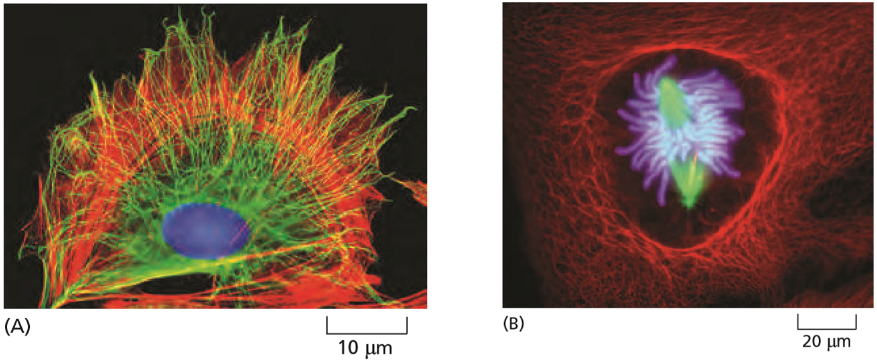
\includegraphics[width = 0.7\textwidth]{1}
	\caption{The cytoskeleton. \textbf{(A)} A cell in culture has been fixed and labeled to show its cytoplasmic arrays of \textbf{microtubules (green)} and \textbf{actin filaments (red)}. \textbf{(B}) This dividing cell has been labeled to show its \textbf{spindle microtubules (green)} and surrounding cage of \textbf{intermediate filaments (red)}. The DNA in both cells is labeled in blue.}
\end{figure}
The cytoskeleton's function depends on three families of protein filaments: 
\begin{itemize}
	\item \textbf{Actin filaments} - determine the shape of the cell’s surface and are necessary for whole-cell locomotion. Moreover they drive the pinching of one cell into two. 
	
	\item \textbf{Microtubules} determine the positioning of membrane-enclosed organelles, direct intracellular transport, and form the mitotic spindle that segregates chromosomes during cell division.
	
	\item \textbf{Intermediate filaments} provide mechanical strength. There exists many differed kinds which are cell specific. 
\end{itemize}
All of these cytoskeletal filaments interact with hundreds of \textbf{accessory proteins that regulate and link} the filaments to other cell components, as well as to each other. \textbf{\gls{motorproteins}} are a type of accessory proteins. They convert the energy of ATP hydrolysis into mechanical force that can either \textbf{move organelles along the filaments} or \textbf{move the filaments themselves}.\\
\\
In differentiated epithelial cells, the cytoskeleton supports both dynamic and stable structures. It \textbf{maintains surface features like \gls{microvilli}} despite continuous remodeling. Moreover, the cytoskeleton also \textbf{establishes cell polarity}, distinguishing the apical and basolateral surfaces to support specialized functions.

\indent As shown in Figure~\ref{polarization_cyto}, \textbf{actin filaments (red) form microvilli} at the apical surface to enhance nutrient absorption and create a \textbf{circumferential belt for cell adhesion}. \textbf{Intermediate filaments (blue) anchor cells} via desmosomes and hemidesmosomes, while \textbf{microtubules (green) organize intracellular transport}. These components together maintain the specialized structure and function of epithelial cells.

\begin{ExWithTitle}{Cell Division - The Cytoskeleton is dynamic}
	An important example of rapid \textbf{cytoskeletal reorganization occurs during cell division}. \textbf{Figure~\ref{cell_division_cyto}} shows a crawling fibroblast with a polarized, dynamic \textbf{actin cytoskeleton (red)}, supported by a \textbf{microtubule cytoskeleton (green)}. During division, the polarized (interphase) microtubule array reorganizes into a bipolar mitotic spindle, which aligns and segregates the duplicated \textbf{chromosomes (brown)}. At the same time, the actin structures that drive fibroblast movement are reorganized, causing the cell to round up and stop migrating. \\
	\indent \textbf{Actin and the motor protein myosin then assemble into a contractile ring} around the cell’s midpoint. This ring constricts to divide the cell in two. Once division is complete, the cytoskeletons of the daughter cells return to their interphase organization, restoring the flattened, motile shape of the original cell.
\end{ExWithTitle}

\begin{figure}[H]
	\centering
	\subfigure[Diagram of changes in cytoskeletal organization associated with cell division.]{
		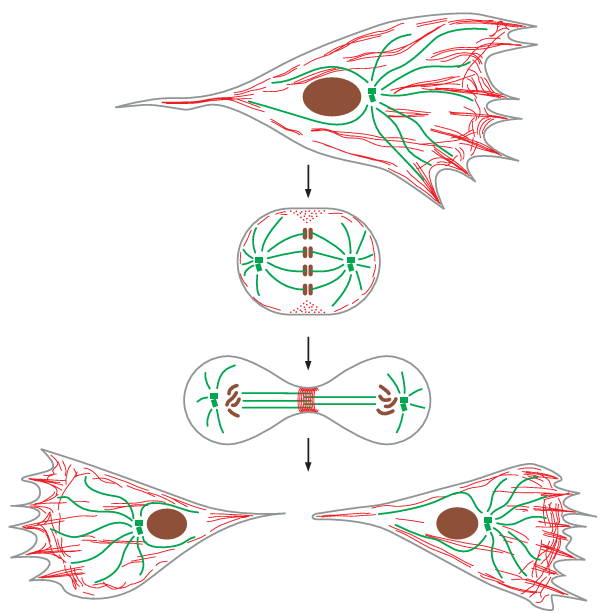
\includegraphics[width = 0.45 \textwidth]{2}
		\label{cell_division_cyto}
	}
	% Second subfigure
	\subfigure[Organization of the cytoskeleton in polarized epithelial cells.]{
		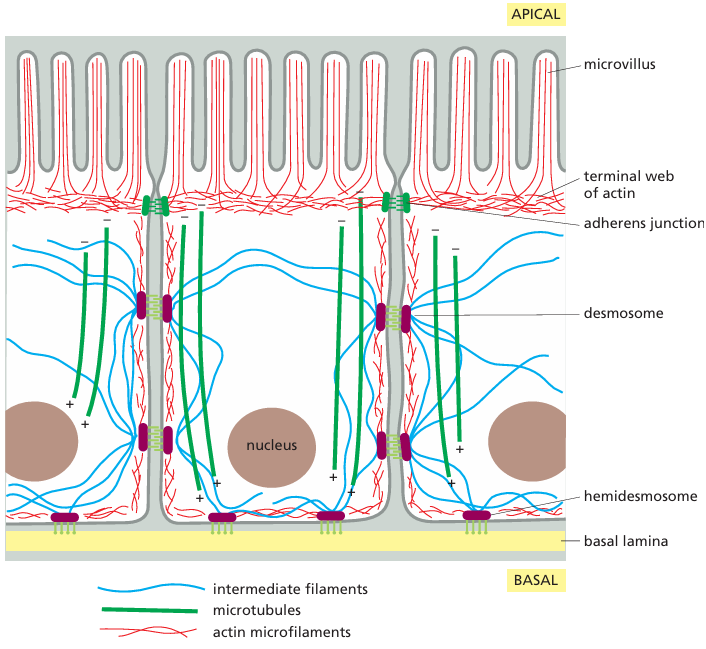
\includegraphics[width = 0.5 \textwidth]{3}
		\label{polarization_cyto}
	}
	\caption{Cytosceleton is dynamic and determines cellular organization and polarization}
\end{figure}

\subsection{Actin Filaments}
\textbf{Actin filaments}, also known as \textit{microfilaments}, are \textbf{helical polymers of the protein actin}. These flexible structures, about 8nm in diameter, assemble into \textbf{linear bundles, networks, and gels}. They are dispersed throughout the cell but are especially concentrated in the \textbf{cell cortex}. 

Actin filaments determine the \textbf{shape of the cell surface}, are essential for \textbf{whole-cell movement}, and play a key role in \textbf{cytokinesis}, where they drive the pinching of one cell into two. 

Their organization supports diverse actin-based structures, including \textit{stress fibers} that anchor to \textit{focal adhesions}, \textbf{cell cortex} (dense, gel-like network of \gls{actinfilaments}), the \textit{lamellipodium} for broad, sheet-like protrusions, the \textit{filopodium} for slender, finger-like extensions, and the contractile apparatus of striated muscle. See fig. \ref{actin_forms} \\
\\
As shown in Figure \ref{actin-monomer} the actin monomer has a nucleotide (\textbf{either ATP or ADP}). \textit{Note that newly synthesized actin filaments still contain ATP as hydrolysis to ADP is slower than the assembly of a new filament.} \\
\indent These monomers then arrange into a filament consisting of two protofilaments, that are held together by lateral contacts. These \textbf{2 protofilaments} wind around each other as two parallel strands of a \textbf{helix} with a twist repeating every 37 nm. Note that every subunits within the filament have the \textbf{same orientation}, thus forming an minus and a plus end. 

\begin{figure}[H]
	\centering
	\subfigure[Structure of an actin monomer and actin filament]{
		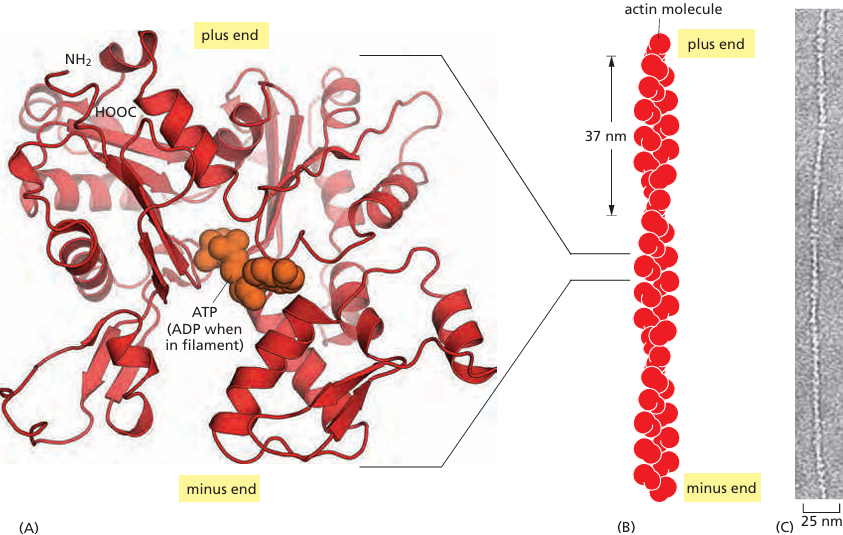
\includegraphics[width = 0.48 \textwidth]{6}
		\label{actin-monomer}
	}
	% Second subfigure
	\subfigure[Actin filaments comes in many forms]{
		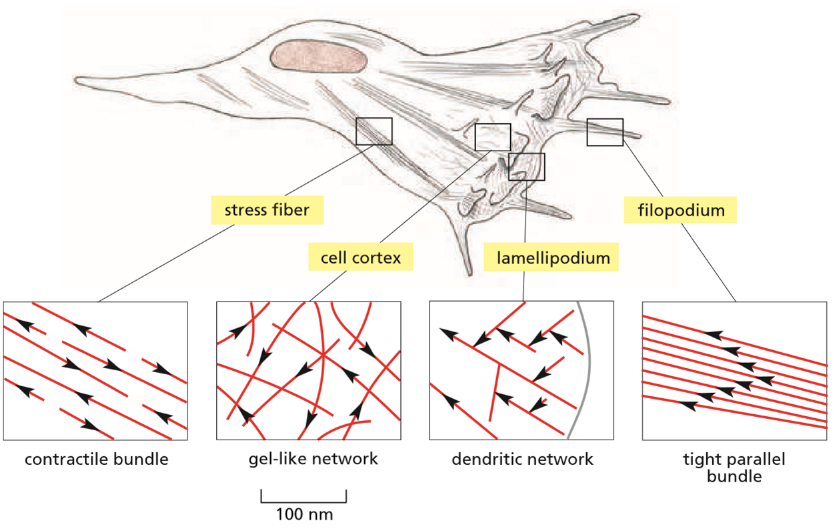
\includegraphics[width = 0.48 \textwidth]{5}
		\label{actin_forms}
	}
	\caption{Actin Filaments}
\end{figure}

\subsubsection{Actin and Actin-Binding Proteins}

\begin{figure}[H]
	\centering
	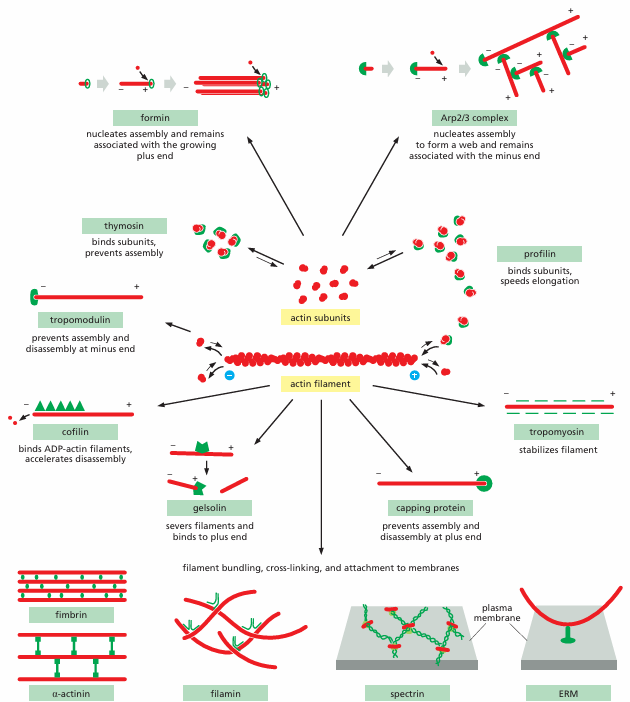
\includegraphics[width = 0.8 \textwidth]{16}
	\caption{Some of the major accessory proteins of the actin cytoskeleton. (Except Myosin and Motor Proteins)}
\end{figure}

\paragraph{Regulation of Actin Filament Formation}
The \textbf{regulation} of action filament formation is an important mechanism by which cells control their shape and movement. This is largely archived by exploring the following effects: 

\subparagraph{Nucleation is the Rate-Limiting Step}
\noindent When polymerization is initiated, \textbf{kinetic barrier to nucleation} results in a \textbf{lag phase}, followed by a phase of \textbf{rapid elongation}. Finally, as the concentration of actin declines, the system approches a \textbf{steady state}. This point is called the \textbf{critical concentration C\textsubscript{c}}.

\begin{RemarkWithTitel}{Barrier to Nucleation}
	A helical polymer is stabilized by multible contacts between adjacent subunits. In the case of actin, two actin molecules bind relatively weakly to each other and thus disassemble quickly. But the \textbf{addition of a third actin monomer} forming a trimer makes the entire group more stable. This creates a barrier to nucleation. 
\end{RemarkWithTitel}

\begin{RemarkWithTitel}{Critical Concentration C\textsubscript{c}}
	C\textsubscript{c} is the concentration of free subunits at which the rate of subunit addition to a filament equals the rate of subunit loss, resulting in a steady-state polymer length. It is defined by the ratio of kinetic rate constants:
	\[
	C_{\text{c}} = \frac{k_{\text{off}}}{k_{\text{on}}} = K_d = \frac{1}{K_{\text{eq}}}
	\]
\end{RemarkWithTitel} 
 
\begin{figure}[H]
	\centering
	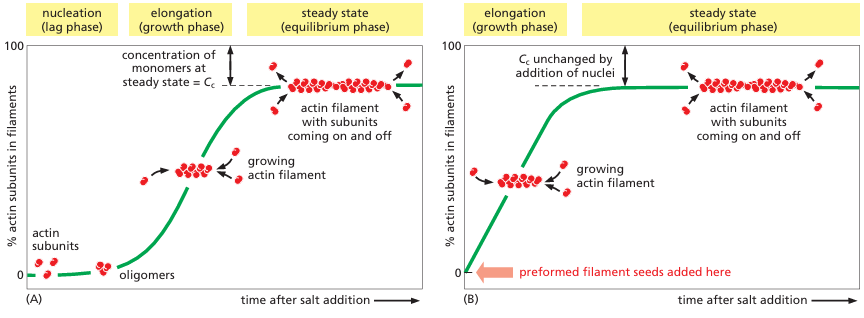
\includegraphics[width = 0.9\textwidth]{7}
	\caption{The time course of actin polymerization in a test tube.}
	\label{}
\end{figure}

\subparagraph{ATP Hydrolysis Within Actin Filaments Leads to Treadmilling at Steady State - Thymosin and Profilin}
Actin filaments are \textbf{polar structures}, meaning their two ends are structurally and functionally distinct: the \textbf{plus (barbed) end grows faster} than the \textbf{minus (pointed) end}. This polarity arises from the uniform orientation of actin monomers within the filament.

When ATP-bound actin monomers add to a filament, they preferentially bind to the plus end due to faster kinetics. Once incorporated, the \textbf{ATP is hydrolyzed to ADP}, a process that occurs more efficiently within the filament. As a result, a \textbf{nucleotide gradient} forms: ATP-actin (T-form) at the plus end and ADP-actin (D-form) toward the minus end.

This hydrolysis does not cause immediate disassembly, but it \textbf{weakens the interactions} between subunits. As a result, D-form actin has a \textbf{higher critical concentration ($C_c$)} than T-form, meaning it dissociates more readily.

At intermediate monomer concentrations, this leads to \textbf{treadmilling}:
\begin{itemize}
	\item The plus end remains in T-form and grows (since monomer concentration $>$ $C_c$ for T-form).
	\item The minus end, being in D-form, shrinks (monomer concentration $<$ $C_c$ for D-form).
\end{itemize}
Thus, the filament maintains a constant length while subunits cycle through it—\textbf{powered by ATP hydrolysis and enabled by filament polarity}. This dynamic turnover is essential for many cellular processes, such as cell movement and shape changes.	
\begin{figure}[H]
	\centering
	\subfigure[Treadmilling of an actin filament]{
		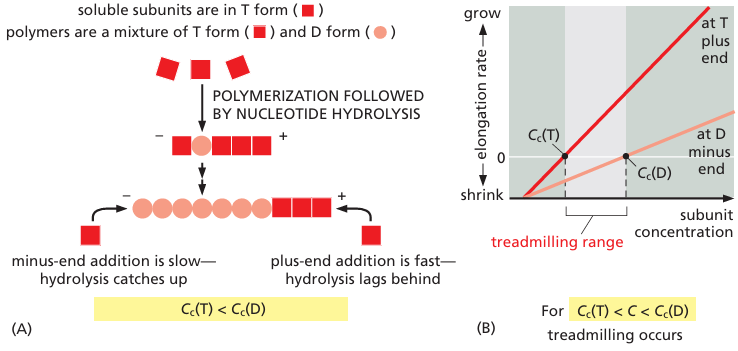
\includegraphics[width = 0.6 \textwidth]{8}
	}
	% Second subfigure
	\subfigure[Structural Polarity]{
		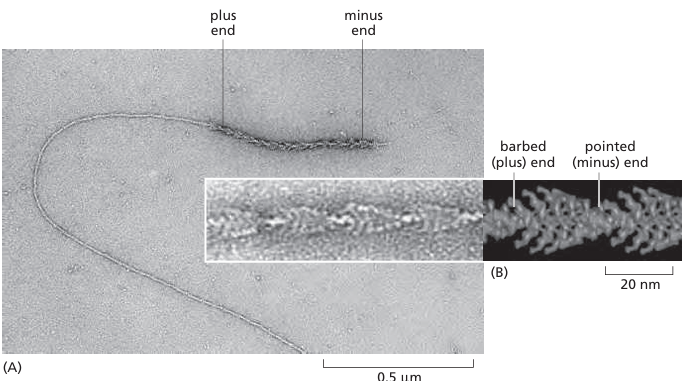
\includegraphics[width = 0.36 \textwidth]{15}
		\label{polarization_cyto}
	}
	\caption{Cytosceleton is dynamic and determines cellular organization and polarization}
\end{figure}

\subparagraph{Monomer Availability Controls Actin Filament Assembly}
Only about half of the actin in non-muscle vertebrate cells is polymerized into filaments. This is largely due to the action of monomer-binding proteins that sequester actin and inhibit spontaneous polymerization. The most abundant of these is \textbf{\gls{thymosin}, which binds actin monomers and holds them in an inactive state}: they cannot polymerize, hydrolyze ATP, or exchange their nucleotide.

In contrast \textbf{\gls{profilin} is used to make actin monomers available} for filament assembly. Profilin which binds the opposite side of the actin monomer from the ATP-binding cleft. Note that profilin \textbf{blocks association with the minus end of filaments}. Upon encountering a filament plus end, the profilin–actin complex adds a monomer, and profilin is released and recycled. 

Since \textbf{thymosin and profilin compete} for binding to actin monomers, the cell can regulate actin assembly by locally modulating profilin activity.

\begin{figure}[H]
	\centering
	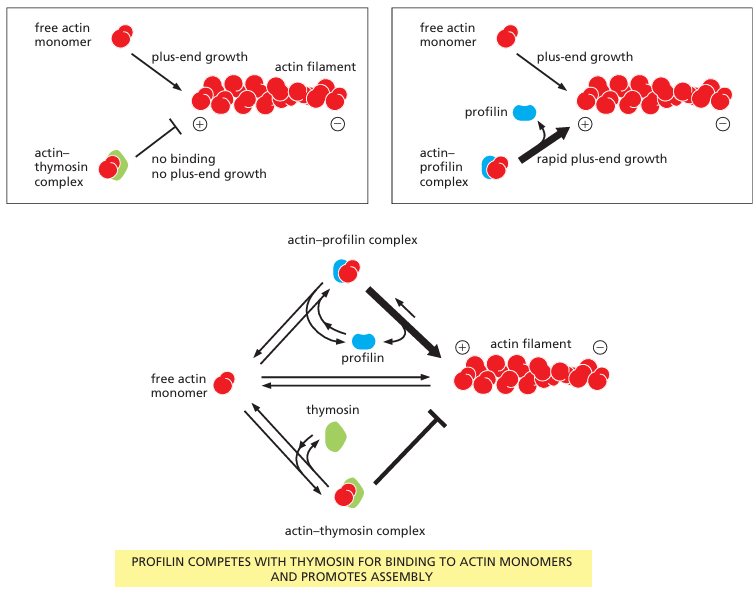
\includegraphics[width = 0.65 \textwidth]{9}
	\caption{ Effects of thymosin and profilin on actin polymerization.}
\end{figure}

\textbf{Profilin activity is spatially and temporally controlled} through phosphorylation and interactions with acidic membrane phospholipids. This targeting is especially important at the plasma membrane, where extracellular signals can recruit profilin to promote localized filament growth, enabling the extension of actin-based structures like lamellipodia and filopodia.

\subparagraph{Formin-mediated actin filament elongation}
\gls{formin} proteins are dimeric actin nucleators that \textbf{promote the growth of long, unbranched actin filaments.} Each subunit in the formin dimer contains a binding site for monomeric actin, and together, they can nucleate new filament formation by capturing and stabilizing two actin monomers. Formins remain attached to the rapidly growing plus end of the filament, allowing continued subunit addition during elongation. 

Formin-mediated actin nucleation occurs primarily at the \textbf{plasma membrane and contributes to the assembly of parallel actin bundles.} There \textbf{rapid remodeling} is essential for cell movement and response to external stimuli.
\begin{figure}[H]
	\centering
	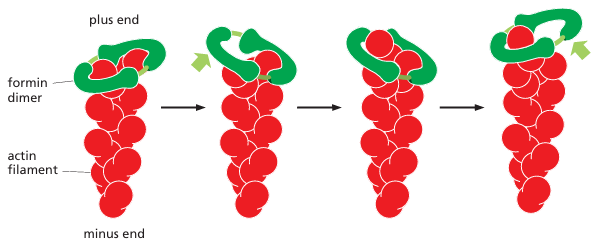
\includegraphics[width = 0.6 \textwidth]{11}
	\label{fig:arp2-3-nucleation}
	\caption{Actin elongation mediated by formins.}
\end{figure}
Some formins have unstructured domains "whiskers" that contain binding sites for profilin. This enhances the growth rate drastically.

\subparagraph{Nucleation of Actin Filaments by the Arp2/3 Complex}
A key requirement for actin polymerization in cells, beyond the availability of actin monomers, is the \textbf{nucleation of new filaments}. This process is \textbf{energetically unfavorable and thus requires specialized proteins to initiate it}. One of the major actin nucleation mechanisms involves the \textbf{\gls{arpcomplex}}, which contains two actin-related proteins (Arp2 and Arp3) that are structurally similar to actin.

In its inactive state, the Arp2/3 complex is held in a conformation that prevents nucleation. Upon activation by nucleation-promoting factors, \textbf{Arp2 and Arp3 are repositioned to mimic the plus end of an actin filament}, enabling actin subunits to assemble and bypass the rate-limiting nucleation step. Importantly, the Arp2/3 complex preferentially nucleates filaments while attached to the side of preexisting actin filaments, forming branches at a 70\textdegree{} angle. 

This branching results in the formation of a dense, treelike actin network that is essential for cell motility and structural organization (see Figure~\ref{fig:arp2-3-nucleation}).

\begin{figure}[H]
	\centering
	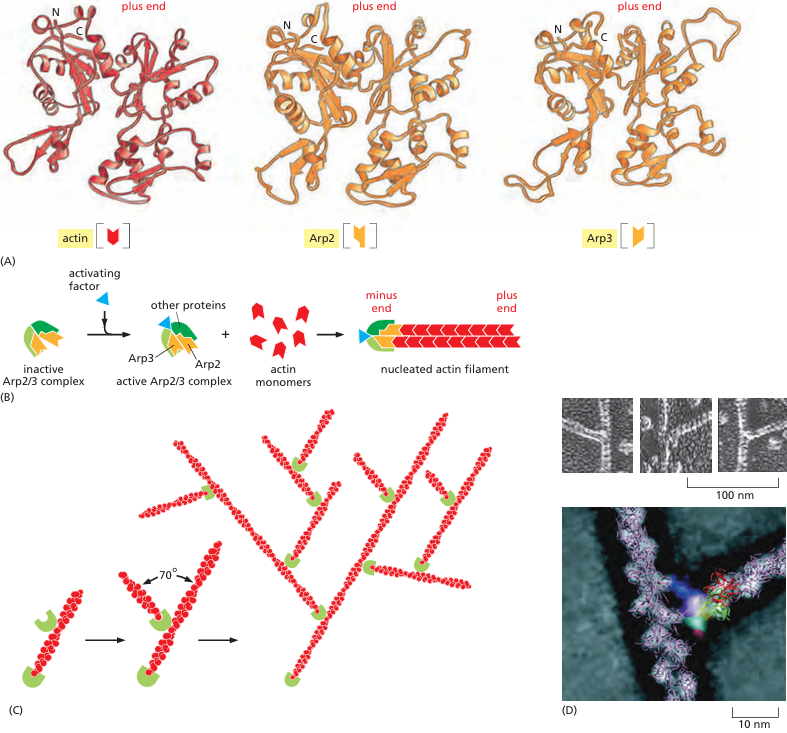
\includegraphics[width = 0.7 \textwidth]{10}
	\caption{Nucleation and actin web formation by the Arp 2/3 complex.}
	\label{fig:arp2-3-nucleation}
\end{figure}

\subparagraph{Actin-Filament-Binding Proteins Alter Filament Dynamics}
Actin filaments are regulated by proteins that bind either \textbf{along their sides or at their ends.}  Figure \ref{capping-actin} show the effect of the presence on the filament dynamics. \textit{Note that Side-binding proteins require high concentrations to coat filaments fully, but end-binding proteins act effectively at low levels, controlling filament dynamics by capping filament ends.} 
\begin{itemize}
	\item  \textbf{\gls{tropomyosin}} binds along filament grooves, stabilizing and \textbf{stiffening filaments} while \textbf{blocking interactions} with other proteins.
	
	\item \textbf{Plus ends} my be capped by \textbf{\gls{CapZ}} caps \textbf{preventing assembly or disassembly}. 
	
	\item \textbf{Minus ends} may be capped by the \textbf{Arp 2/3 complex} or \textbf{\gls{tropomodulin}}, \textbf{preventing assembly or disassembly} 
\end{itemize}


\subparagraph{Severing Proteins Promote Actin Turnover and Cytoskeletal Remodeling}
The dynamic reorganization of actin filaments also depends on proteins that \textbf{sever existing filaments}. Severing creates numerous new filament ends, whose fate depends on local conditions and regulatory proteins. This can dramatically accelerate filament turnover and fluidize the cytoskeleton.

Two key severing factors are \gls{gelsolin} and \gls{cofilin}. 
\begin{enumerate}
	\item \textbf{Gelsolin} is activated by elevated cytosolic Ca2+. It binds the side of an actin filament and inserts itself between subunits when transient thermal fluctuations create small gaps. This results in filament severing. After cleavage, \textbf{gelsolin remains attached to the new plus end}, acting as a \textbf{cap and preventing further polymerization}.
	
	\item \textbf{Cofilin}, also known as \textit{actin depolymerizing} factor, \textbf{binds to ADP-actin filaments twisting them} more tightly and weakening subunit interactions. This mechanical strain increases the likelihood of spontaneous severing and \textbf{accelerates filament disassembly}. Since ATP hydrolysis lags behind filament growth, cofilin spares newer, ATP-rich filaments and selectively dismantles older ones, supporting the polarized actin turnover required for processes like cell migration.
\end{enumerate}

\begin{figure}[H]
	\centering
	\subfigure[Filament capping and its effects on filament dynamics. Red line shows the effect a capping protein]{
		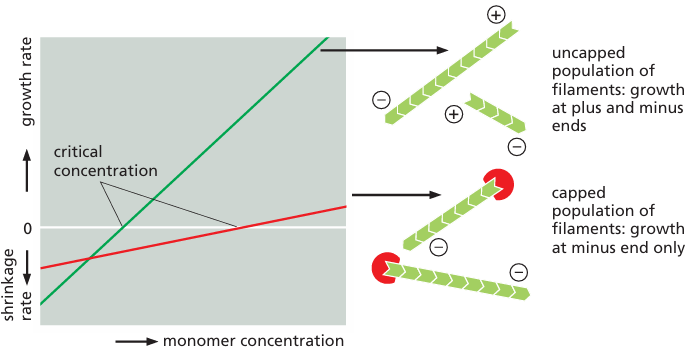
\includegraphics[width = 0.5 \textwidth]{12}
		\label{capping-actin}
	}
	% Second subfigure
	\subfigure[Twisting of an actin filament induced by cofilin.]{
		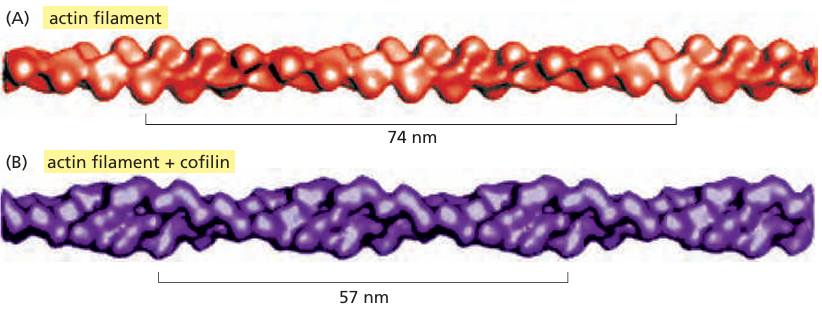
\includegraphics[width = 0.45 \textwidth]{13}
	}
	\caption{Cytosceleton is dynamic and determines cellular organization and polarization}
\end{figure}

\paragraph{Structural Organization of Actin Filaments}
As shown in Figure \ref{actin_forms} there are different forms of structural organization between actin filaments. This depends on specialized \textbf{accessory proteins}. 

There are 2 main types \textbf{bundling proteins}, which cross-link actin filaments into a parallel array, and \textbf{gel-forming proteins}, which hold two actin filaments together in a large angle. 

Note that each type of bundling proteins also \textbf{determines which other molecules can interact} with the cross-linked actin filaments. 

For example, \textbf{Myosin II} is the motor protein that enables stress fires to contract. Thus very close packeding actin filaments cased by the binding protein \textbf{fibrin} exclude myosin and are thus not contractile. But on the other hand \textbf{$\alpha$-actinin} cross-linked oppositely polarized actin filament are more loose bundles, that allow the binding of myosin, creating contractile actin bundles.  See fig. \ref{myosine-boundels}

\begin{figure}[H]
	\centering
	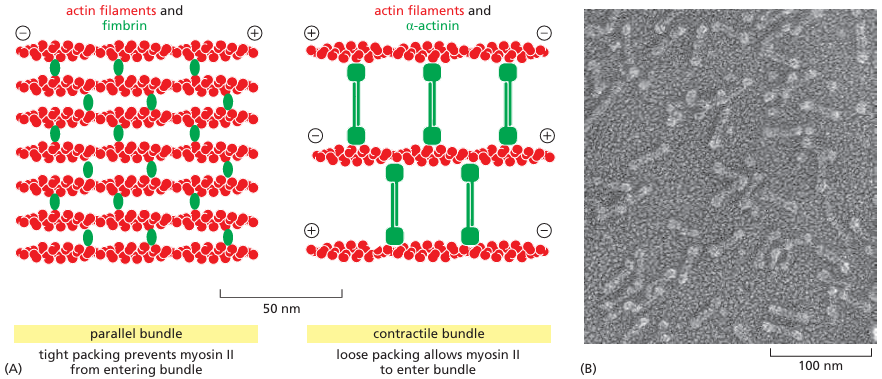
\includegraphics[width = 0.7 \textwidth]{14}
	\caption{The formation of two types of actin filament bundles.}
	\label{myosine-boundels}
\end{figure}

\subsubsection{Myosin Motor Proteins}
Actin-based motor proteins are members of the \textbf{myosin superfamily}. The first motor protein to be identified was skeletal muscle myosin, which generates the force for muscle contraction (\textit{myosin II}). \\
\indent All myosins share a motor domain dark green (see fig \ref{myosinfam}), but their C-terminal tails (light green) and N-terminal extensions (light blue) are divers. \\
\indent Many myosins form dimers , with two motor domains per molecule. \textbf{Myosin VI is unique in moving towards the minus end} (instead of the plus end) of the actin filament. \\
\\
Motor proteins use structural changes in their ATP-binding sites to produce \textbf{cyclic interactions with a cytoskeletal filament}. Each cycle of ATP binding, hydrolysis, and release propels them forward \textbf{in a single direction} to a new binding site along the filament. \textit{Note these changes are asymmetric and designed to move in one direction, based on the polarity, for example myosin II moves towards the plus end.} 
\begin{figure}[H]
	\centering
	\subfigure[Myosin superfamily members.]{
		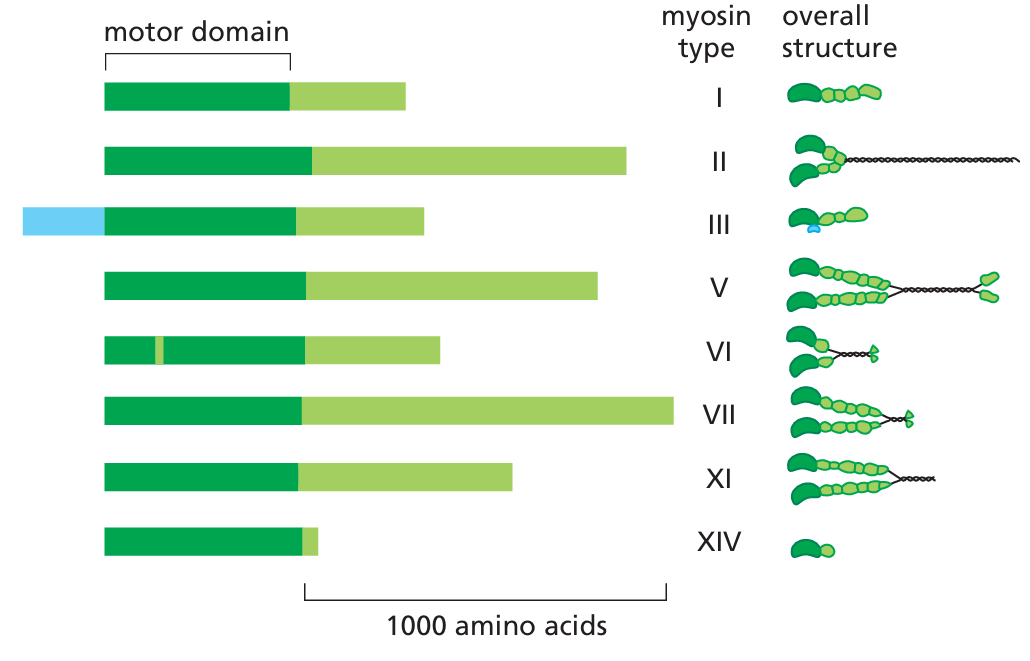
\includegraphics[width = 0.4 \textwidth]{17}
		\label{myosinfam}
	}
	% Second subfigure
	\subfigure[Myosin V carries cargo along actin filaments.]{
		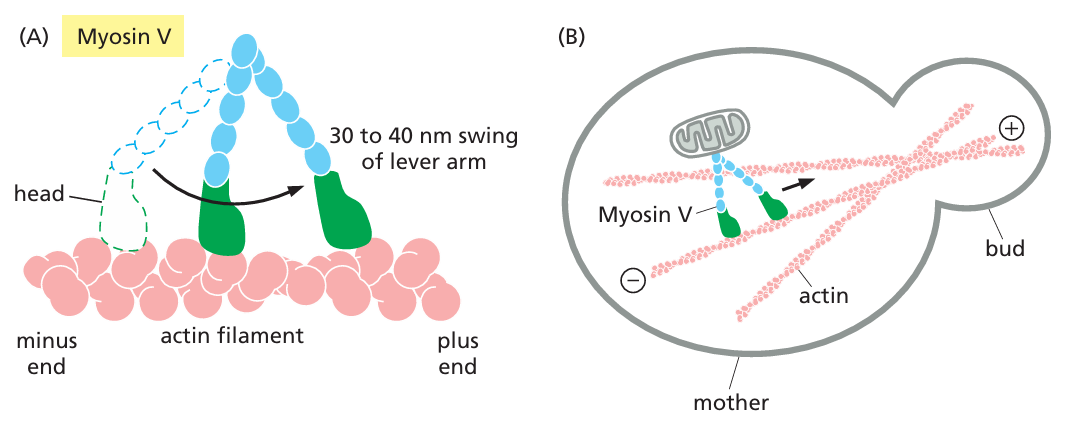
\includegraphics[width = 0.55 \textwidth]{18}
		\label{myosinV}
	}
	\caption{Myosin Motor Proteins}
\end{figure}
\indent \textbf{Myosin V} (see fig \ref{myosinV}) is a two-headed myosin with a large step size and is involved in \textbf{organelle transport} along actin filaments. In contrast to myosin II motors, which work in ensembles and are attached only transiently to actin filaments, myosin V moves continuously along actin  filaments without letting go. Myosin V motors carry a wide range of cargoes including mRNA, ER, and secretory vesicles. \textit{Note that Myosin V takes larger steps then Myosin II.} \\
\\
Most non-muscle cells contain small amounts of contractile actin myosin II bundles that form transiently. These are regulated by \textbf{phosphorylation} (rather then the troponin mechanism in muscle cells). These contractile bundles provide mechanical support to cells, for example, by assembling into cortial \textbf{stress fibres} that connect the cell to the ECM. through focal adhesion.   
\begin{figure}[H]
	\centering
	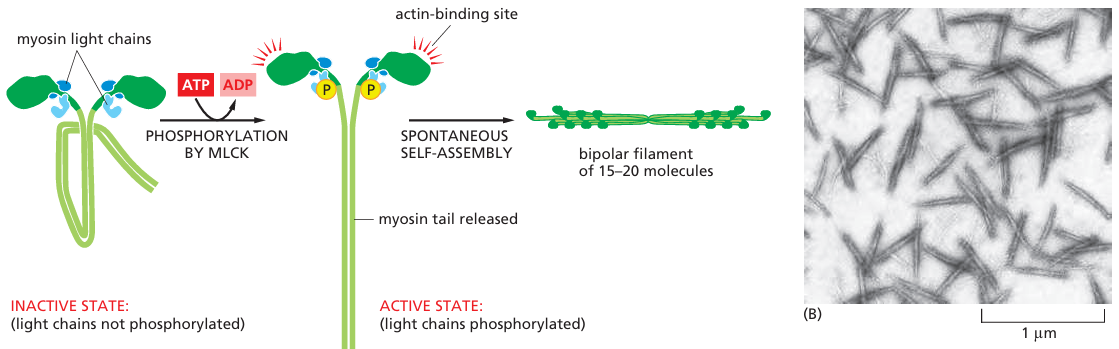
\includegraphics[width = 0.85\textwidth]{19}
	\caption{Light-chain phosphorylation and the regulation of the assembly of myosin II into thick filaments.}
\end{figure}


\subsubsection{Cell Migration via Actin Dynamics}
Cell movement is driven by coordinated forces generated in the actin-rich cortex. At the front of a migrating cell, \textbf{actin polymerization pushes the plasma membrane forward to form a lamellipodium}, which attaches firmly to the substrate via \textbf{focal adhesions}. These adhesions are mediated by \textbf{integrin proteins, which connect the actin cytoskeleton to the extracellular matrix}. As new adhesions form at the leading edge, older ones at the rear are disassembled. \\
\indent Simultaneously, \textbf{myosin-driven contraction at the back of the cell pulls the cell body forward}, relieving tension and generating traction. \\
\indent Actin filaments at the leading edge assemble at their barbed ends, and if not anchored to adhesions, they move rearward due to continued polymerization and myosin activity. When linked to integrins via adaptor proteins, contractile forces are transmitted through the adhesions to produce forward motion. \textbf{This cycle of protrusion, adhesion, contraction, and release allows the cell to move in a stepwise or smooth fashion}.

\begin{figure}[H]
	\centering
	\subfigure[Actin polymerization drives plasma membrane protrusion]{
		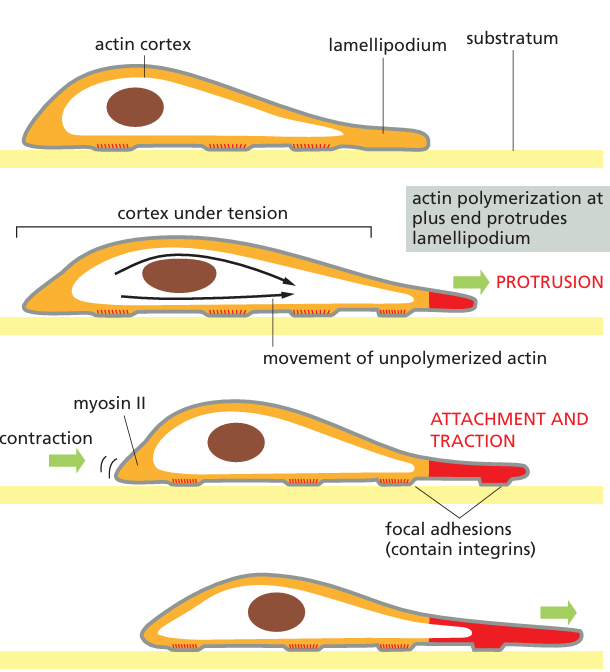
\includegraphics[width = 0.45\textwidth]{42}
	}
	% Second subfigure
	\subfigure[Myosin contraction and cell adhesion allow cells to pull themselves forward]{
		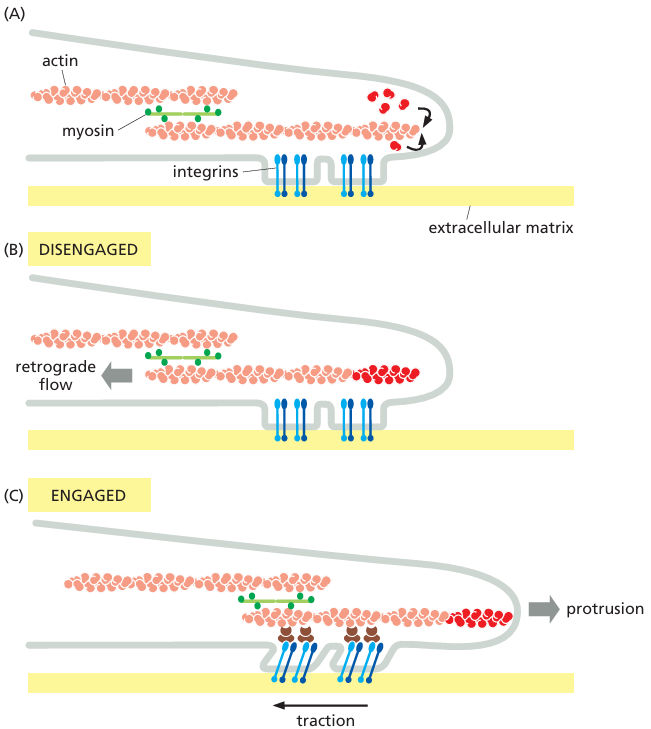
\includegraphics[width = 0.45 \textwidth]{43}
	}
	\caption{Cell Migration via Actin Dynamics}
\end{figure}

\begin{RemarkWithTitel}{Membranes "breathe" thermally, allowing polymerization}
	Once the filament contacts the membrane, there would be no room for a new subunit to it onto the end of the growing chain. It is thought that random thermal motions briefly expose the plus end of the filament, allowing a new subunit to be added. By taking advantage of these small windows of opportunity, actin polymerization acts as a ratchet to capture random thermal motions.
\end{RemarkWithTitel}

\paragraph{The Rho-family}
The small GTPases of the Rho-family Cdc42, Rac, and Rho play distinct roles in organizing the actin cytoskeleton of fibroblasts. 
\begin{itemize}
	\item The activation of \textbf{\gls{Cdc42}} promotes the formation of \textbf{filopodia (thin, finger-like protrusions)} at the cell surface important for sensing and migration.
	
	\item The activation of \textbf{\gls{Rac}} leads to the formation of lamellipodia—broad, \textbf{sheet-like membrane protrusions}— by dense branched actin networks (Arp2/3 complex).
	
	\item The activated \textbf{\gls{Rho}} stimulates the formation of thick \textbf{stress fibers—contractile actin bundles}.
\end{itemize}
\begin{figure}[H]
	\centering
	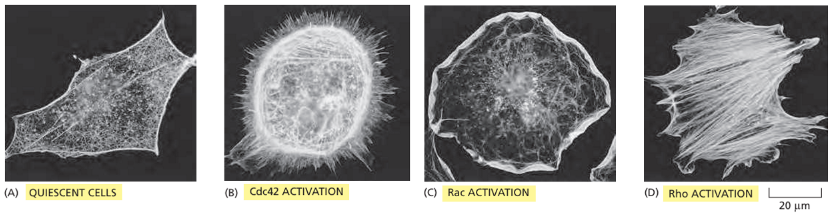
\includegraphics[width = \textwidth]{44}
	\caption{The dramatic effects of Cdc42, Rac, and Rho on actin organization in fibroblasts (visualized through actin staining)}
\end{figure}

Mechanistically, \textbf{Rac-GTP promotes actin branching through activation of the WASp family and the Arp2/3 complex}, while also \textbf{inhibiting myosin II} activity via the PAK kinase pathway, reducing contractility and promoting network formation. \\
\indent Meanwhile, \textbf{Rho-GTP activates formins for actin nucleation} and \textbf{enhances myosin II} contractility via the Rho-associated kinase (Rock), which maintains myosin activation and \textbf{stabilizes actin bundles by inhibiting cofilin}.

\begin{figure}[H]
	\centering
	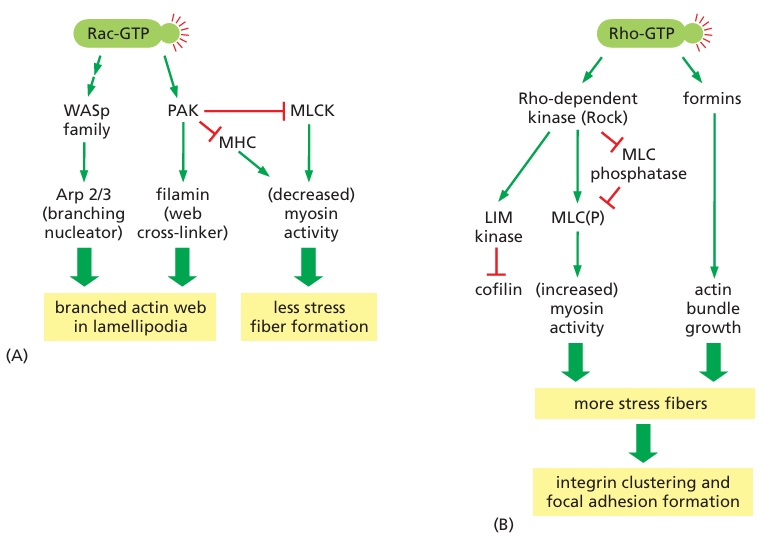
\includegraphics[width = 0.8\textwidth]{45}
	\caption{The contrasting effects of Rac and Rho activation on actin organization.}
\end{figure}



\subsection{Microtubules}
\textbf{Microtubules} determine the positions of membrane-enclosed organelles, direct intracellular transport, and form the mitotic spindle that segregates chromosomes during cell division.\\
\\
Microtubules are structurally more complex than actin filaments, but they are also highly \textbf{dynamic} and play comparably diverse and important roles in the cell. Microtubules are polymers of the protein \textbf{\gls{tubulin}}.  \\
\indent The tubulin subunit is itself a heterodimer formed from two closely related globular proteins called $\alpha$-tubulin and $\beta$-tubulin, which are held tightly together by noncovelent bonds.  Each monomer has a binding site for \textbf{GTP} While the GTP is trapped in the $\alpha$-monomer, the nucleotide on the $\beta$-subuit can be either in the GTP or in GDP form. \\
\\
A \textbf{\gls{microtubules} is hollow tube made from 13 parallel protofilaments.} This creats multiple contacts among subunits make microtubules stiff and difficult to bend. Microtubles can be several millimeters bevor it starts to bend because of thermic motion (persistence length), making microtubules the \textbf{stiffest} and straightest structural elements found in most animal cells. \\
\indent The subunits in each protofilament point in the same direction, and the protofilaments itself are aligned parallel. Therefore, the microtubule lattice itself has a distinct structural \textbf{polarity}, which \textbf{$\alpha$-tubulins exposed at the minus end and $\beta$-tubulins expoised at the plus end}. 
\begin{figure}[H]
	\centering
	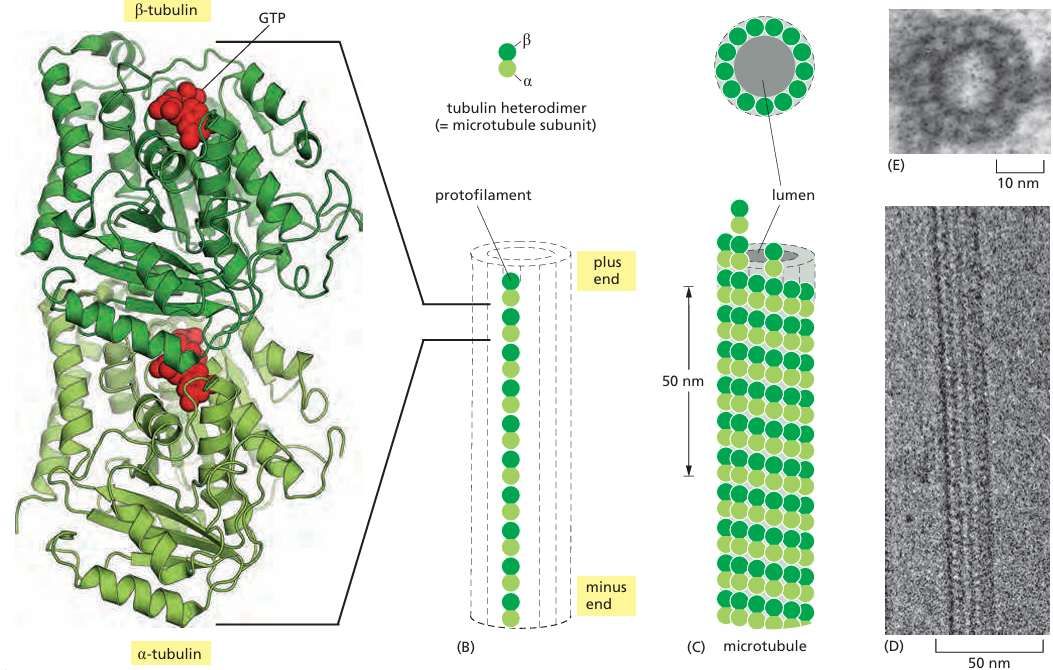
\includegraphics[width = 0.7\textwidth]{21}
	\caption{The structure of a microtubule and its subunit.}
\end{figure}

Microtubules undergo dynamic instability with the \textbf{plus end ($\beta$) shrinking and growing more rapidly.} These dynamics, like those of actin filaments, are influenced by the binding and hydrolysis of nucleotide - GTP in this case. \\
\indent GTP hydrolysis occurs only within the $\beta$-tubulin subunit, plus end of dimer. It proceeds very slowly in free tubulin subunits but is accelerated when they are incorporated into microtubules. Following GTP hydrolysis, the free phosphate group is released and 
the GDP remains bound to $\beta$-tubulin within the microtubule lattice. Therefore it exists the \textbf{D-form} and the \textbf{T-form}. Because of the differences in structure, the T-form tends to polymerize and the D-form to depolymerize. \\
\indent A growing strand has GTP cap (multiple in T forms at the end). Now if the rate of subunit addition is low, hydrolysis may occur before the next subunit is added, and the tip of the filament will then be in the D form. This would induce depolymerization. This process is called \textbf{dynamic instability} and is dependent on the free concentration. See fig. \ref{dynamic-instability}

\begin{figure}[H]
	\centering
	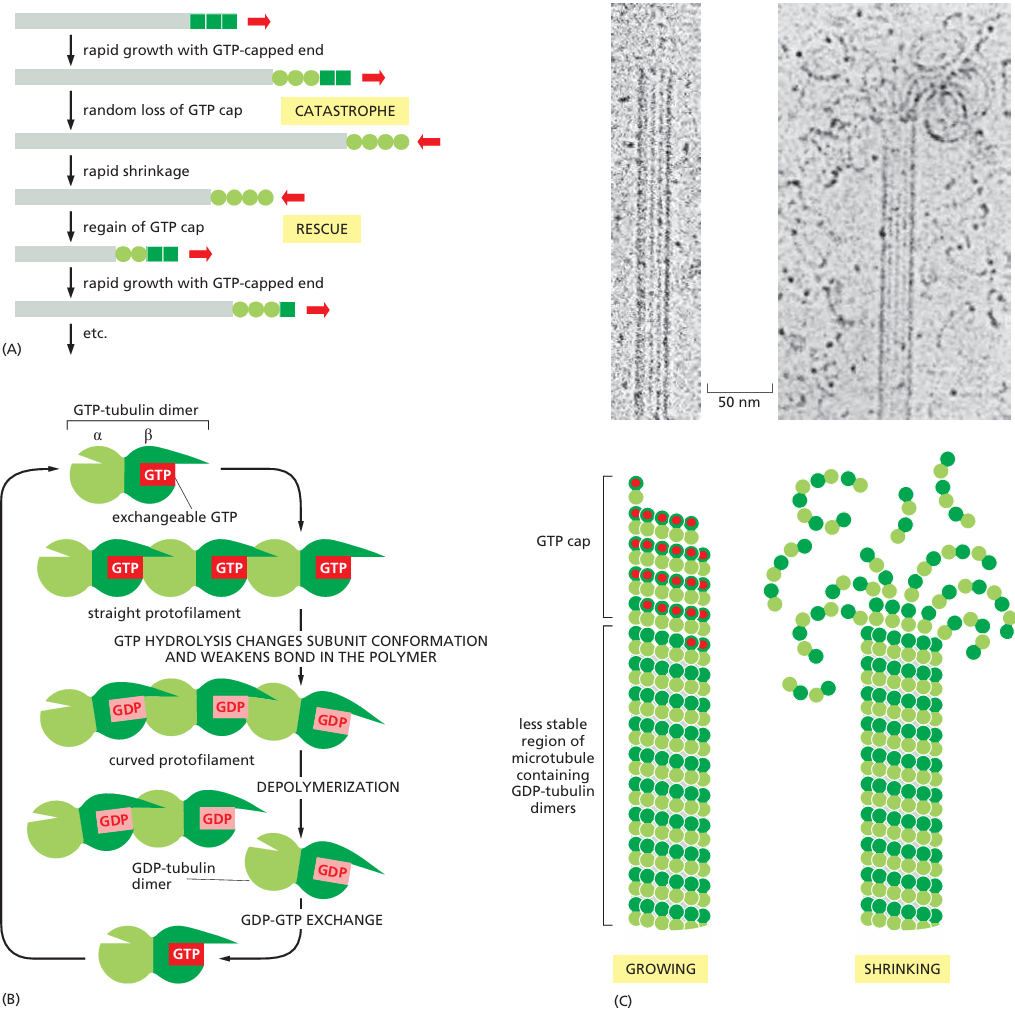
\includegraphics[width = 0.8\textwidth]{22}
	\caption{Dynamic instability due to the structural differences between a growing and a shrinking microtubule end.}
	\label{dynamic-instability}
\end{figure}

\subsubsection{Tubuli binding proteins}

\begin{figure}[H]
	\centering
	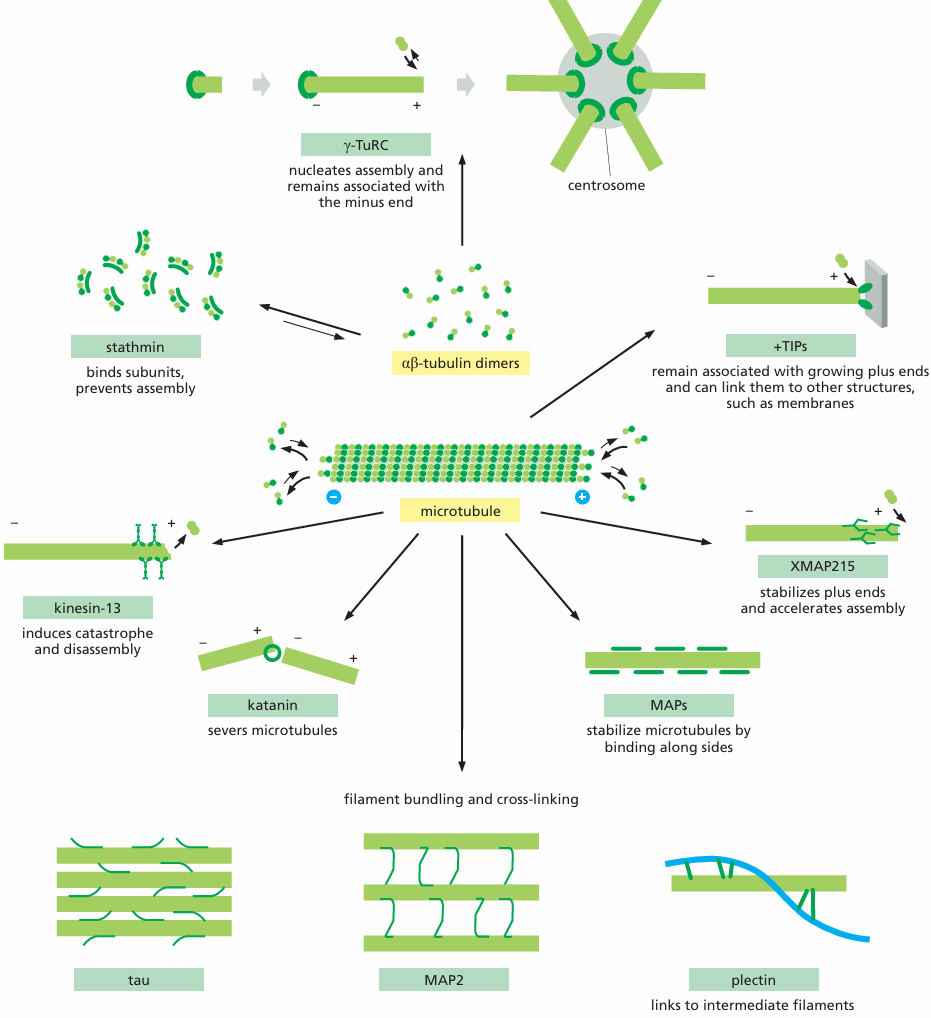
\includegraphics[width = 0.8\textwidth]{20}
	\caption{Some of the major accessory proteins of the microtubule cytoskeleton.}
\end{figure}

\paragraph{Regulation of Microtubule Formation}

Microtubule formation requires the assembly of many tubulin heterodimers, so spontaneous nucleation demands a very high concentration of subunits. To overcome this, cells use specialized factors to facilitate nucleation. \textbf{$\gamma$-tubulin} is essential for initiating microtubule growth. \\
\indent $\gamma$-Tubulin is concentrated at the \textbf{microtubule-organizing center (MTOC)}, the site where nucleation typically occurs. There, it forms part of the \textbf{\gls{gammaturc}}, which acts as a template for microtubule assembly. The $\gamma$-TuRC includes accessory proteins that arrange $\gamma$-tubulin into a spiral ring structure, matching the 13-protofilament architecture of a growing microtubule. \textit{Side note, $\gamma$-tubulin are one of the most conserved proteins out there}

\begin{figure}[H]
	\centering
	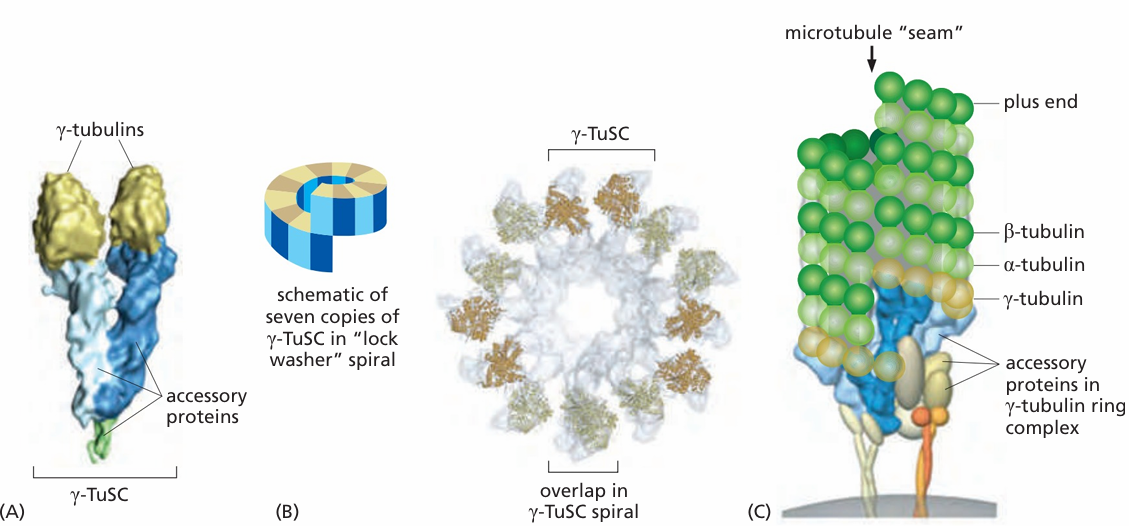
\includegraphics[width = 0.7 \textwidth]{25}
	\caption{Microtubule nucleation by the $\gamma$-tubulin ring complex.}
\end{figure}


There are other proteins that are involved in regulating the transition between microtubule growth and shrinkage. A few of them bind to the end of the microtubule promoting (de-)polymerization. \textbf{See fig. \ref{endbinding}}
\begin{itemize}
	\item \textbf{catastrophe factors} like \gls{kinesin13} destabilize and promote depolymerization. \textbf{Kinesin 13} is a member of the kinesin superfamily of motor proteins, but it does not transport cargo. Instead, it binds to the ends of microtubules and promotes depolymerization, increasing microtubule catastrophe frequency. It plays key roles in mitosis, especially in spindle dynamics and chromosome segregation.
	
	\item \textbf{Microtubule-Assosiated Proteins (MAPs)} sutch as \textbf{XMAP215} stabilize the end of growing microtubule and promote polymerization. \gls{xmap215} binds to tubulin dimers and delivers them to the growing plus end of microtubules, thereby promoting microtubule growth. XMAP215 is crucial for regulating microtubule dynamics during interphase and mitosis. 
\end{itemize}
 
\begin{figure}[H]
	\centering
	\subfigure[The effects of proteins that bind to microtubule ends.]{
		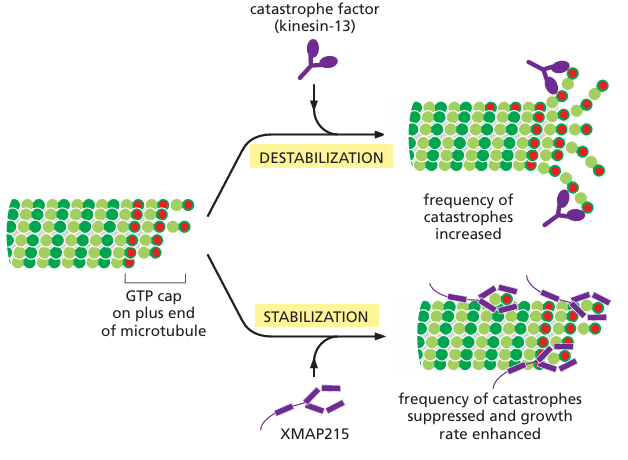
\includegraphics[width = 0.6 \textwidth]{23}
		\label{endbinding}
	}
	% Second subfigure
	\subfigure[Sequestration of tubulin by stathmin.]{
		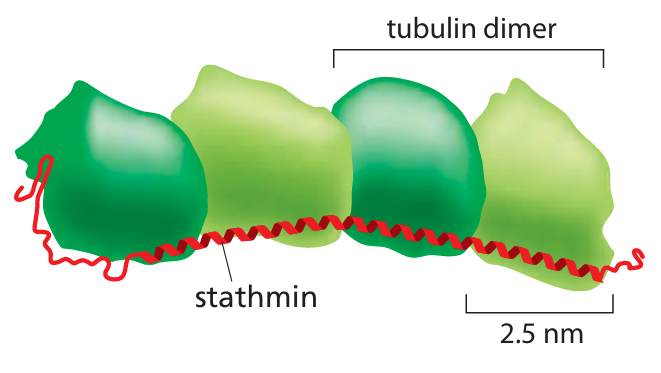
\includegraphics[width = 0.35 \textwidth]{24}
		\label{stathmin}
	}
	\caption{Kinesin 13, XMAP215, and Stathmin regulate the formation of microtubule.}
\end{figure}

An other posibility to regulate the formation of mcrotubule is to \textbf{mess with the concentration of tubulin} like it was done for actin filaments. The cell sequesters unpolymerized tubulin subunits to maintain a pool of active subunits at a level near the critical concentration (like for actin). \\ 
\indent One molecule of the small protein \textbf{\gls{stathmin} (see fig. \ref{stathmin})} binds to two tubulin heterodimers and prevents their addition to the ends of microtubules, thus \textbf{reducing the effective concentration of tubulin}. Therefore it enhances the likelihood that a growing to microtubule will switch to the shrinking state. Its activity is controlled by phosphorylation. 


\paragraph{Microtubules Originate from the Centrosome in Animal Cells}
The \textbf{\gls{centrosome} is the major microtubule-organizing center (MTOC)} in most animal cells. It is located near the nucleus and consists of a \textbf{pair of orthogonally arranged \gls{centriole} surrounded by \gls{pcm}}.  This protein-rich matrix anchors $\gamma$-tubulin ring complexes ($\gamma$-TuRCs), which nucleate microtubules. \\
\indent The minus ends of microtubules are embedded in the centrosome, $\gamma$-TuRC, while plus ends extend outward into the cytoplasm , forming a dense array.
\begin{figure}[H]
	\centering
	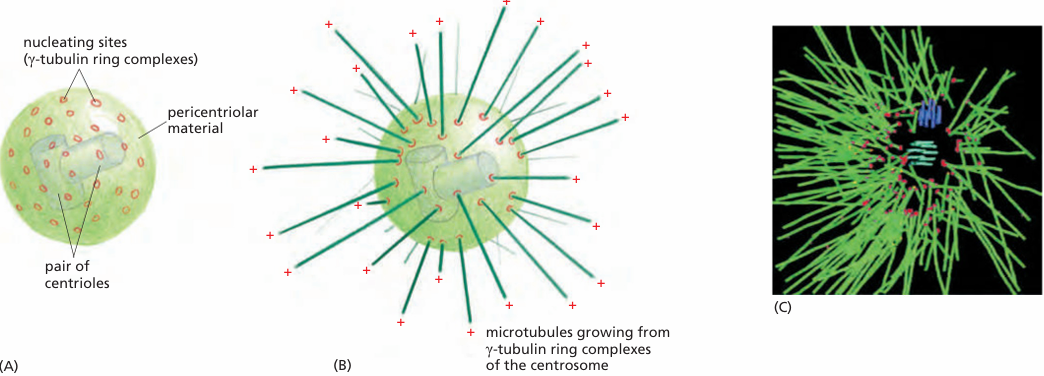
\includegraphics[width = 0.7 \textwidth]{26}
	\caption{The centrosome}
\end{figure}

The centrioles are cylindrical cellular structures composed of nine triplet microtubules arranged with ninefold symmetry. his structural symmetry is guided by the \textbf{\gls{SAS-6}} protein, which assembles into a ring at the core of the cartwheel structure. See fig. \ref{pairOfcentrioles} (d)\\
\indent Centrioles are found in pairs (\textbf{the mother and daughter centrioles}) within the centrosome. During the cell cycle, centrioles \textbf{duplicate} and play a key role in spindle formation during mitosis. They can also act as basal bodies to initiate the formation of \textbf{cilia and flagella}. 

\begin{figure}[H]
	\centering
	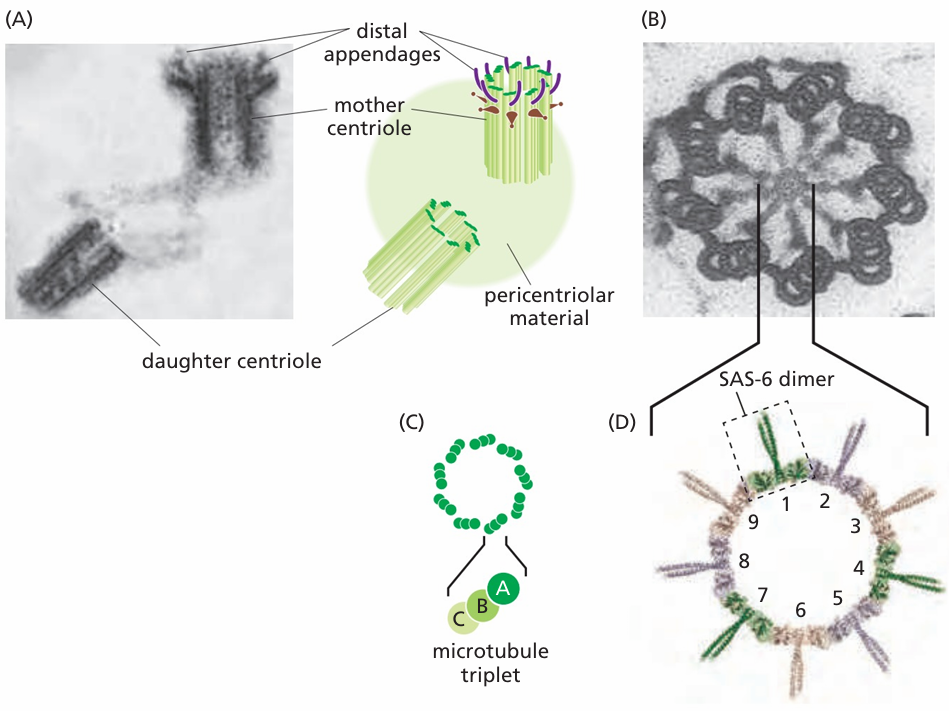
\includegraphics[width = 0.7 \textwidth]{27}
	\caption{A pair of centrioles in the centrosome.}
	\label{pairOfcentrioles}
\end{figure}

Remarkably, even without a centrosome, microtubules can self-organize. After physically severing part of a fish pigment cell, the microtubules in the detached fragment reorganize, \textbf{clustering their minus ends at the center, forming a new MTOC} (see fig. \ref{self-organizing}). This shows that microtubules can establish cellular polarity and coordinate internal architecture independently, highlighting their self-organizing capability.

\begin{figure}[H]
	\centering
	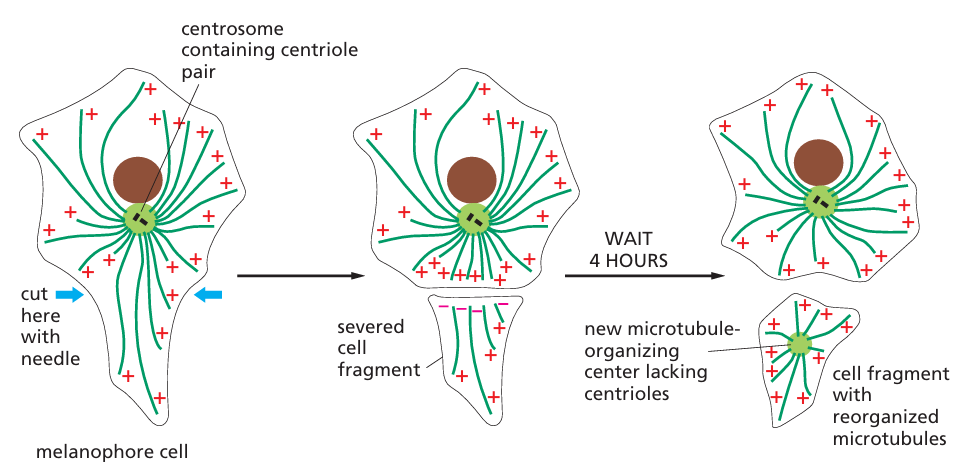
\includegraphics[width = 0.7 \textwidth]{28}
	\caption{A microtubule array can find the center of a cell.}
	\label{self-organizing}
\end{figure}

\paragraph{Organization of Microtubules}
\textbf{Microtubule-associated proteins (MAPs)} stabilize microtubules and mediate their interactions with other cellular structures. These proteins have one domain that binds to the microtubule surface and another that projects outward, affecting microtubule spacing.\\
Figure \ref{organizationMAPs} ilustrats how MAPs organize microtubule bundles. 
\begin{itemize}
	\item \textbf{\gls{MAP2}} has a \textbf{long projecting domain}, allowing it to cross-link microtubules at wider distances, resulting in \textbf{widely spaced bundles}.
	
	\item \textbf{\gls{tau}}, with a shorter projecting domain, creates more closely packed bundles.
\end{itemize}

\begin{figure}[H]
	\centering
	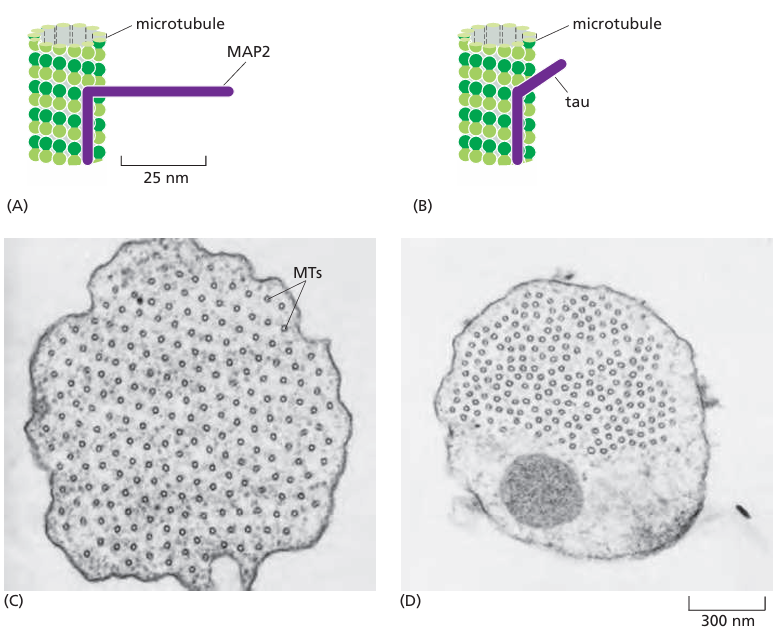
\includegraphics[width = 0.7 \textwidth]{29}
	\caption{Organization of microtubule bundles by MAPs.}
	\label{organizationMAPs}
\end{figure}


\begin{RemarkWithTitel}{Microtubule organization in a neuron}
	In a neuron, microtubule organization is complex. In the \textbf{axon, all microtubules share the same polarity} with the plus end pointing towards the axon terminus. But \textbf{no single microtubles stretches the entire lenght of the axon}: instead, \textbf{short overlapping segments} of parallel microtubules make the tracks for fast axonal transport. \\
	\indent In the \textbf{dendrites, the microtubules are of mixed polarity}. Vesicles can associate with both kinesin and dynein and move in either direction along the microtubules in axons and dendrites. \\
	\indent \textit{Note in neurons, abnormal tau aggregation is associated with neurodegenerative diseases such as Alzheimer's.}
\end{RemarkWithTitel}


\subsubsection{Motor Proteins associated with Tubuli}
Like actin filaments, microtubules also use motor proteins to transport cargo and perform a variety of other functions within the cell. There are two major classes of microtubule-based motors, \textbf{kinesins and dyneins}.

\paragraph{Kinesins}
Kinesin is a class of motor proteins that move generally \textbf{along microtubules towards the plus end, but not all}. \\
\indent Like myosin, \gls{kinesin} is a member of a large protein superfamily, for which the motor domain is the common element. Despite this conserved region, kinesins differ significantly in the position of the motor domain and the function of their tail domains, leading to a range of specialized roles within the cell.\\
\indent \textbf{Kinesin-5} forms a bipolar tetramer that slides two microtubule past each other, much like the bipolar filaments of myosin II. \textbf{Kinesin-13}, with a central motor domain, lacks conventional motility and instead promotes microtubule depolymerization at the ends. \textbf{Kinesin-14} contains a C-terminal motor and moves toward the minus end of microtubules, opposite to most kinesins.\\
\\
\textbf{Kinesin-1}, is one of the best understood members. It is a dimeric motor protein composed of two motor domains (heads) connected via a coiled-coil tail. It walks along microtubules using a coordinated “hand-over-hand” stepping mechanism that allows for processive movement, meaning it can take many steps without detaching from the microtubule. \textbf{See fig. \ref{mechanochemical-kinesin}} \\
\indent At the beginning of a step, the \textbf{lagging head} is tightly bound to the microtubule and carries \textbf{ATP}, while the \textbf{front head} is loosely attached with \textbf{ADP} in its binding site. ATP binding to the leading head triggers a conformational change in a flexible region called the \textbf{neck linker}, which shifts forward. This movement propels the lagging head past the leading head.\\
\indent Once the lagging head detaches (following ATP hydrolysis and phosphate release), it swings forward and rebinds to a new tubulin site as the new leading head. Meanwhile, the previous leading head becomes the new rear head, preparing for another cycle. This alternating cycle ensures continuous, directional transport of cargo along microtubules.

\begin{figure}[H]
	\centering
	\subfigure[Kinesin and kinesin related proteins.]{
		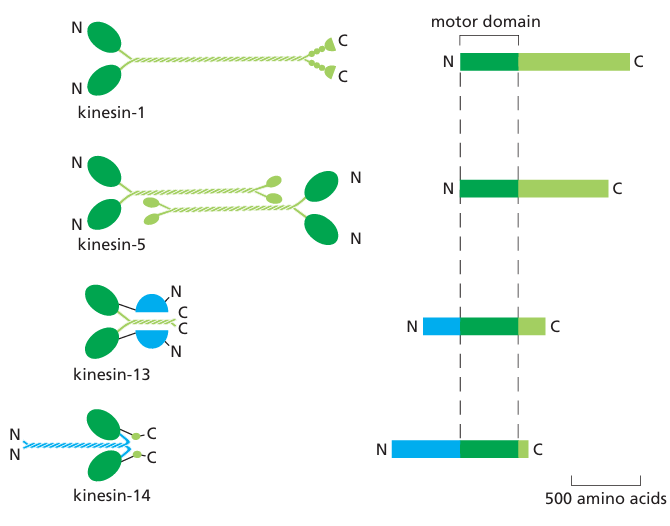
\includegraphics[width = 0.6 \textwidth]{30}
	}
	% Second subfigure
	\subfigure[The mechanochemical cycle of kinesin.]{
		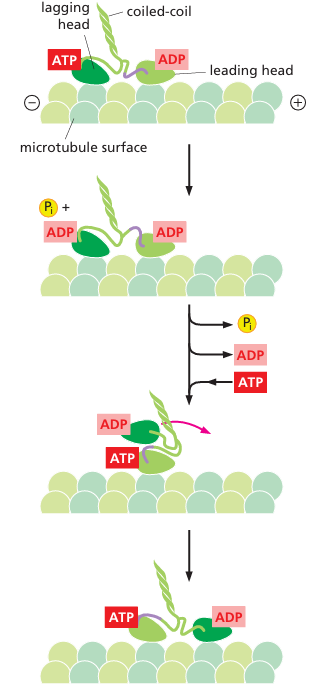
\includegraphics[width = 0.25\textwidth]{31}
		\label{mechanochemical-kinesin}
	}
	\caption{Kinesin 13, XMAP215, and Stathmin regulate the formation of microtubule.}
\end{figure}

\paragraph{Dyneins}
\gls{dynein} is a class of motor proteins that move \textbf{along microtubules towards the minus end}. They are structurally different from kinesin or mysoin.\\
\indent \textbf{cytoplasmic dynein} is a two-headed molecule, with each head formed by a separate heavy chain. Notably, the dynein motor head is \textbf{considerably larger} than those of myosin or kinesin. See fig. \ref{cytoplasmic-dynein}\\
\\
Each dynein heavy chain contains domains responsible for ATP hydrolysis and microtubule binding, organized around a large motor domain composed of a ring of \textbf{six AAA} (ATPases Associated with diverse cellular Activities) domains. Of these, \textbf{only one retains full ATPase activity} (dark red). From this motor ring, a coiled-coil stalk projects to bind microtubules, while a tail domain connects dynein to its cargo \textit{or, in the case of axonemal dyneins, to an adjacent microtubule.}\\
\indent\textbf{ Dynein’s movement is powered by ATP hydrolysis}. In the ATP-bound state, the stalk detaches from the microtubule. Upon hydrolysis, the stalk reattaches, and release of ADP and phosphate triggers a large conformational change (involving the\textbf{ rotation of the head and the stalk relative to the tail}) —\textbf{the power stroke}— which moves the cargo or slides adjacent microtubules. 

\begin{figure}[H]
	\centering
	\subfigure[cytoplasmic dynein]{
		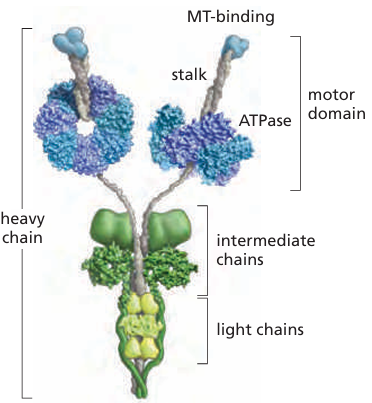
\includegraphics[width = 0.3\textwidth]{32}
		\label{cytoplasmic-dynein}
	}
	% Second subfigure
	\subfigure[The power stroke of dynein.]{
		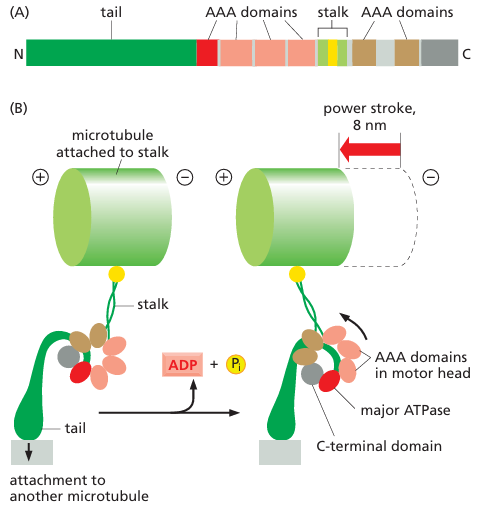
\includegraphics[width = 0.55\textwidth]{33}
		\label{mechanochemical-kinesin}
	}
	\caption{Dynein}
\end{figure}

\textbf{\gls{dynactin}} mediates the attachment of dynein to a membrane
enclosed organelle (\textbf{See fig. \ref{Dynactin}}). Dynein requires the presence of a large number of \textbf{accessory proteins to associate with membraneenclosed organelles}. Dynactin is a large complex that includes components that bind weakly to microtubules, components that bind to dynein itself, and components that form a small, actin-like filament made of the actin-related protein Arp1.

\begin{RemarkWithTitel}{Regulated melanosome movements in fish pigment cells.}
	In certain fish species, pigment cells regulate skin coloration by actively transporting large pigment granules called melanosomes. These movements are triggered by hormonal or neuronal signals that alter intracellular cyclic AMP (cAMP) levels.\\
	\indent The \textbf{melanosome are moved along microtubules using motor proteins}. This dynamic transport system allows rapid and reversible changes in cell appearance, contributing to color adaptation. \textbf{See fig \ref{fishfishfish}}
\end{RemarkWithTitel}

\begin{figure}[H]
	\centering
	\subfigure[Dynactin mediates the attachment of dynein to a membrane enclosed organelle.]{
		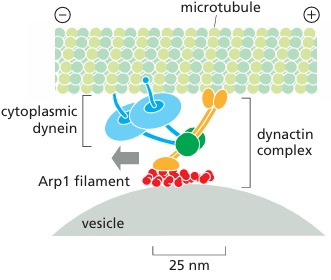
\includegraphics[width = 0.35 \textwidth]{34}
		\label{Dynactin}
	}
	% Second subfigure
	\subfigure[Regulated melanosome movements in fish pigment cells.]{
		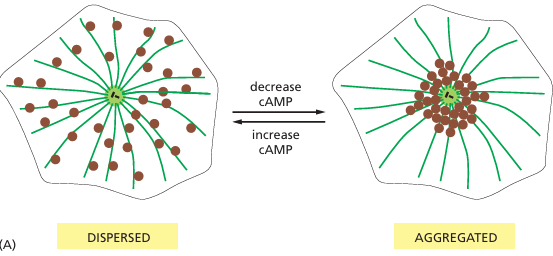
\includegraphics[width = 0.6\textwidth]{35}
		\label{fishfishfish}
	}
	\caption{}
\end{figure}

\subsubsection{Celia and Fagella}
Cilia and flagella are highly specialized and efficient \textbf{motility structures built from microtubules and dynein}. Both cilia and agella are hairlike cell appendages that have a bundle of microtubules at their core. \textbf{Flagella}, found on sperm and protozoa, move with an \textbf{undulating motion} (like a snake) to propel cells through liquid. \textbf{Cilia} beat in a \textbf{whip-like}, breaststroke motion to move cells or fluids across tissue surfaces, such as mucus in the respiratory tract or eggs in the oviduct.\\
\indent Inside a cilium and a flagellum is a \textbf{microtubule-based cytoskeleton called the \gls{axoneme}}. This consists of nine outer doublet microtubules arranged in a ring around two central singlet microtubules (\textbf{9 + 2}). Along the length of the axoneme, linking projections between microtubules occur at regular intervals to maintain structural integrity and enable coordinated bending. See fig. \ref{flagandcili}
\begin{figure}[H]
	\centering
	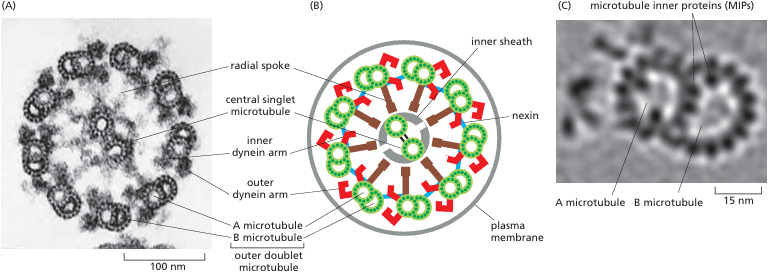
\includegraphics[width = 0.8\textwidth]{36}
	\caption{The arrangement of microtubules in a flagellum or cilium.}
	\label{flagandcili}
\end{figure}

\textbf{Axonemal dynein} forms bridges between neighboring microtubule doublets in the axoneme. When activated, dynein motors attempt to "walk" along adjacent doublets, \textbf{generating a sliding force}. However, if linking proteins between the doublets prevent sliding, the fore will be converted into a \textbf{bending motio}n—the basis for ciliary and flagellar beating.
\begin{figure}[H]
	\centering
	\subfigure[Ciliary dynein.]{
		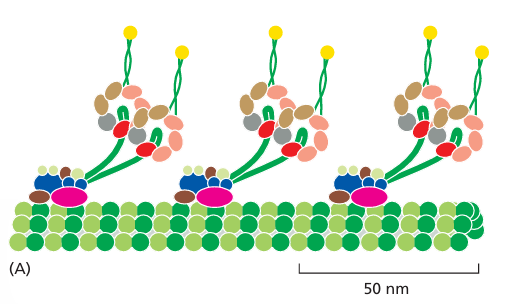
\includegraphics[width = 0.35 \textwidth]{39}
	}
	% Second subfigure
	\subfigure[The bending of an axoneme.]{
		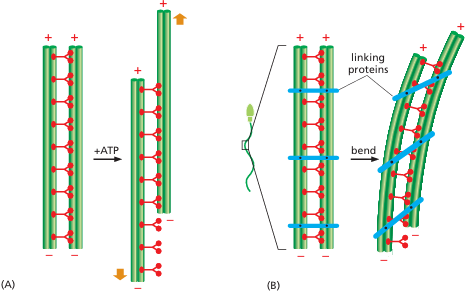
\includegraphics[width = 0.6\textwidth]{37}
	}
	\caption{Movement of cilia and flagella}
\end{figure}

The \textbf{\gls{primarycilium}} is a non-motile, \textbf{antenna-like structure} present on nearly all vertebrate cells. Though structurally similar to motile cilia, it serves primarily as a \textbf{sensory organelle}, detecting signals from the external environment. Built from a \textbf{basal body derived from the mother centriole}, the primary cilium \textbf{grows during interphase} and is \textbf{resorbed before cell division}.\\
\indent Its internal structure—the axoneme—is assembled and maintained through \textbf{intraflagellar transport (IFT)}, using kinesin-2 and cytoplasmic dynein 2 to move proteins and lipids in and out. Primary cilia are essential for functions such as smell and vision, therefore the structure is very \textbf{rich in signaling molecules} (like hedgehog signaling components).

\begin{figure}[H]
	\centering
	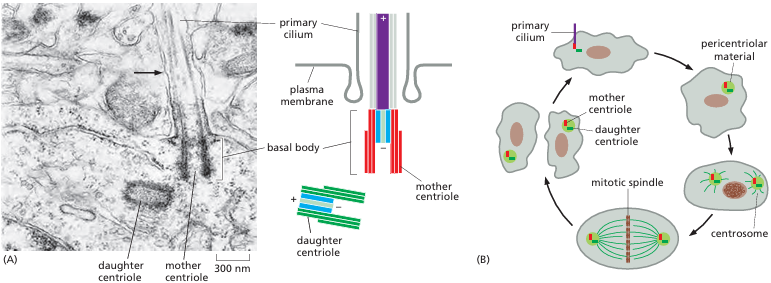
\includegraphics[width = 0.9 \textwidth]{38}
	\caption{Primary cilia.}
\end{figure}

\subsection{Intermediate filaments}

\gls{intermediatefilaments} are a type of \textit{cytoskeletal protein}. They provide \textbf{mechanical strength} to cells, particularly those under stress. These filaments evolved from \textbf{nuclear lamins}, which form a supportive mesh under the nuclear envelope and are present in most eukaryotes. Unlike actin and tubulin, which are highly conserved, \textbf{intermediate filaments are diverse}, encoded by around 70 different genes in humans with cell-type-specific roles.\\
\\
Intermediate filament (IF) structure is built from elongated proteins with a central $\alpha$-helical domain that forms coiled-coil dimers. Two dimers align antiparallel to form tetramers, the building blocks of IFs. Unlike actin or tubulin, IF subunits \textbf{lack nucleotide-binding sites and have no structural polarity}. Tetramers pack laterally into eight-protofilament bundles, resulting in a \textbf{strong, flexible, ropelike filament}. \textit{While IFs are very stable, some types (like vimentin) are dynamic in cells, with phosphorylation regulating their disassembly.} \\
\indent These filaments are crucial for cellular processes that involve shape changes, like division, migration, and differentiation

\begin{figure}[H]
	\centering
	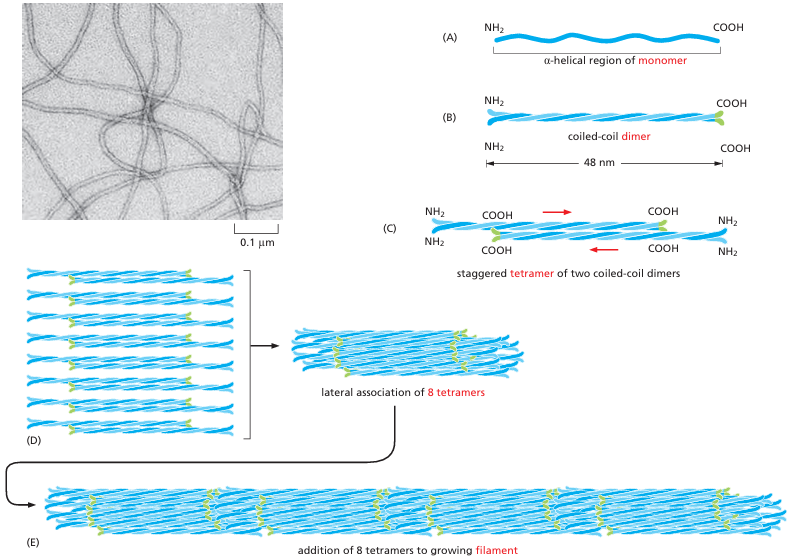
\includegraphics[width = 0.9 \textwidth]{40}
	\caption{A model of intermediate filament construction.}
\end{figure}

\subsubsection{Keratins (not the gym bro stuff)}

\gls{keratins} are the most diverse family of intermediate filaments, with 54 types identified in humans. They are primarily found in \textbf{epithelial cells, hair, and nails.} These filaments provide mechanical strength to epithelial tissues and \textbf{persist even after cell death, forming structures like skin, hair, and nails.}\\
\indent Keratin expression patterns are clinically \textbf{important in diagnosing and treating epithelial cancers}. In cells, keratin filaments anchor at desmosomes and hemidesmosomes to reinforce tissue structure, and proteins like filaggrin help bundle them, contributing to skin toughness. Mutations in filaggrin are linked to dry skin diseases such as eczema.

\begin{RemarkWithTitel}{Blistering of the skin caused by a mutant keratin gene.}
	Mutations in keratin genes cause several genetic diseases characterized by fragile skin and other tissues. For example, \textit{epidermolysis bullosa simplex} results from \textbf{defective keratins in the basal layer of the epidermis}, causing skin to blister even under minor mechanical stress due to cell rupture. \\
	\indent \textit{These mutations disrupt keratin filament assembly, particularly when they alter the ends of the protein’s central rod domain, leading to cytoskeletal disorganization and increased cell fragility.}

	\begin{figure}[H]
		\centering
		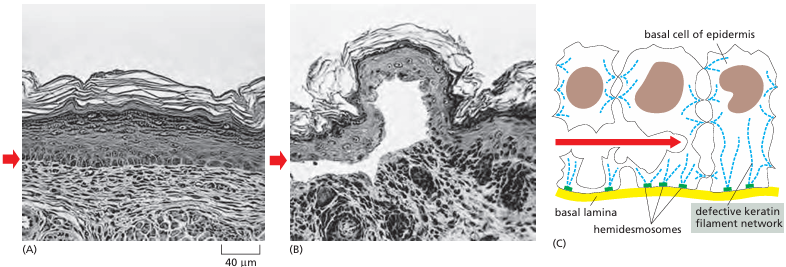
\includegraphics[width = 0.9 \textwidth]{41}
		\caption{Blistering of the skin caused by a mutant keratin gene.}
	\end{figure}
\end{RemarkWithTitel}

	
\end{document}